\documentclass[t,11pt,aspectratio=169]{beamer}
\usepackage{tikz}
\usepackage{pgfplots}
\usetikzlibrary{calc}
\usepackage[utf8]{inputenc}
\usepackage[ngerman]{babel}
\usepackage{amsmath,amsfonts,amssymb}
\usepackage{framed}
\usecolortheme{orchid}
\usepackage{etoolbox}
\useinnertheme[shadow=true]{rounded}

\usepackage{verbatim}

%%% PROGRESSBAR
\definecolor{pbblue}{HTML}{D8D8D8}% filling color for the progress bar
\definecolor{pbgray}{HTML}{F2F2F2}% background color for the progress bar
\useoutertheme{infolines}
\setbeamerfont{footline}{size=\normalsize}
\setbeamersize{text margin left=30pt,text margin right=30pt}
\makeatletter
\setbeamertemplate{footline}
{
	\leavevmode%
	\hbox{%
		\begin{beamercolorbox}[wd=.333333\paperwidth,ht=2.5ex,dp=1ex,center]{title in head/foot}%
			\usebeamerfont{title in head/foot}\insertshorttitle
		\end{beamercolorbox}%
		\begin{beamercolorbox}[wd=.333333\paperwidth,ht=2.5ex,dp=1ex,center]{date in head/foot}%
			%\usebeamerfont{date in head/foot}\insertshortdate{}\hspace*{2em}
			%\insertframenumber\hspace*{2ex} 
		\end{beamercolorbox}
		\begin{beamercolorbox}[wd=.333333\paperwidth,ht=3ex,dp=1ex,center]{author in head/foot}%
			\usebeamerfont{author in head/foot}\insertshortauthor~~%\beamer@ifempty{\insertshortinstitute}{}{(\insertshortinstitute)}
		\end{beamercolorbox}%
	}%
	\vskip0pt%
}
\makeatother
\makeatletter
\def\progressbar@progressbar{} % the progress bar
\newcount\progressbar@tmpcounta% auxiliary counter
\newcount\progressbar@tmpcountb% auxiliary counter
\newdimen\progressbar@pbht %progressbar height
\newdimen\progressbar@pbwd %progressbar width
\newdimen\progressbar@tmpdim % auxiliary dimension
\progressbar@pbwd=\linewidth
\progressbar@pbht=1.5ex
\def\progressbar@progressbar{%
    \progressbar@tmpcounta=\insertpagenumber
    \progressbar@tmpcountb=\insertdocumentendpage
    \progressbar@tmpdim=\progressbar@pbwd
    \multiply\progressbar@tmpdim by \progressbar@tmpcounta
    \divide\progressbar@tmpdim by \progressbar@tmpcountb
  \begin{tikzpicture}[rounded corners=3pt,very thin]
    \shade[top color=pbgray!20,bottom color=pbgray!20,middle color=pbgray!50]
      (0pt, 0pt) rectangle ++ (\progressbar@pbwd, \progressbar@pbht);
      \shade[draw=pbblue,top color=pbblue!50,bottom color=pbblue!50,middle color=pbblue] %
        (0pt, 0pt) rectangle ++ (\progressbar@tmpdim, \progressbar@pbht);
    \draw[color=normal text.fg!50]  
      (0pt, 0pt) rectangle (\progressbar@pbwd, \progressbar@pbht) 
        node[pos=0.5,color=normal text.fg] {\textnormal{%
             \pgfmathparse{\insertpagenumber*100/\insertdocumentendpage}%
             \pgfmathprintnumber[fixed,precision=0]{\pgfmathresult}\,\%%
        }%
    };
  \end{tikzpicture}%
}
\addtobeamertemplate{headline}{}
{%
  \begin{beamercolorbox}[wd=\paperwidth,ht=4ex,center,dp=1ex]{white}%
    \progressbar@progressbar%
  \end{beamercolorbox}%
}
\makeatother

\setbeamertemplate{frametitle}[default][center]

%%% BLOCKS
% block = Aufgabe
\setbeamercolor{block title}{fg=black,bg=blue!30!white} 
\setbeamercolor{block body}{fg=black, bg=blue!3!white}

% alertblock = Definition
\setbeamercolor{block title alerted}{fg=black,bg=red!50!white} 
\setbeamercolor{block body alerted}{fg=black, bg=red!3!white}

% exampleblock = Wiederholung
\setbeamercolor{block title example}{fg=black,bg=green!30!white} 
\setbeamercolor{block body example}{fg=black, bg=green!3!white}

\setbeamercovered{transparent}
\setbeamertemplate{navigation symbols}{}

\addtocounter{page}{-1}
\addtocounter{framenumber}{-1}
\setbeamercovered{invisible}





\begin{document}
	
\begin{frame}
    Schiefetypen
	\begin{center}
		\begin{tabular}{ccc}
			linkssteil / rechtsschief & symmetrisch & rechtssteil / linksschief  \\
			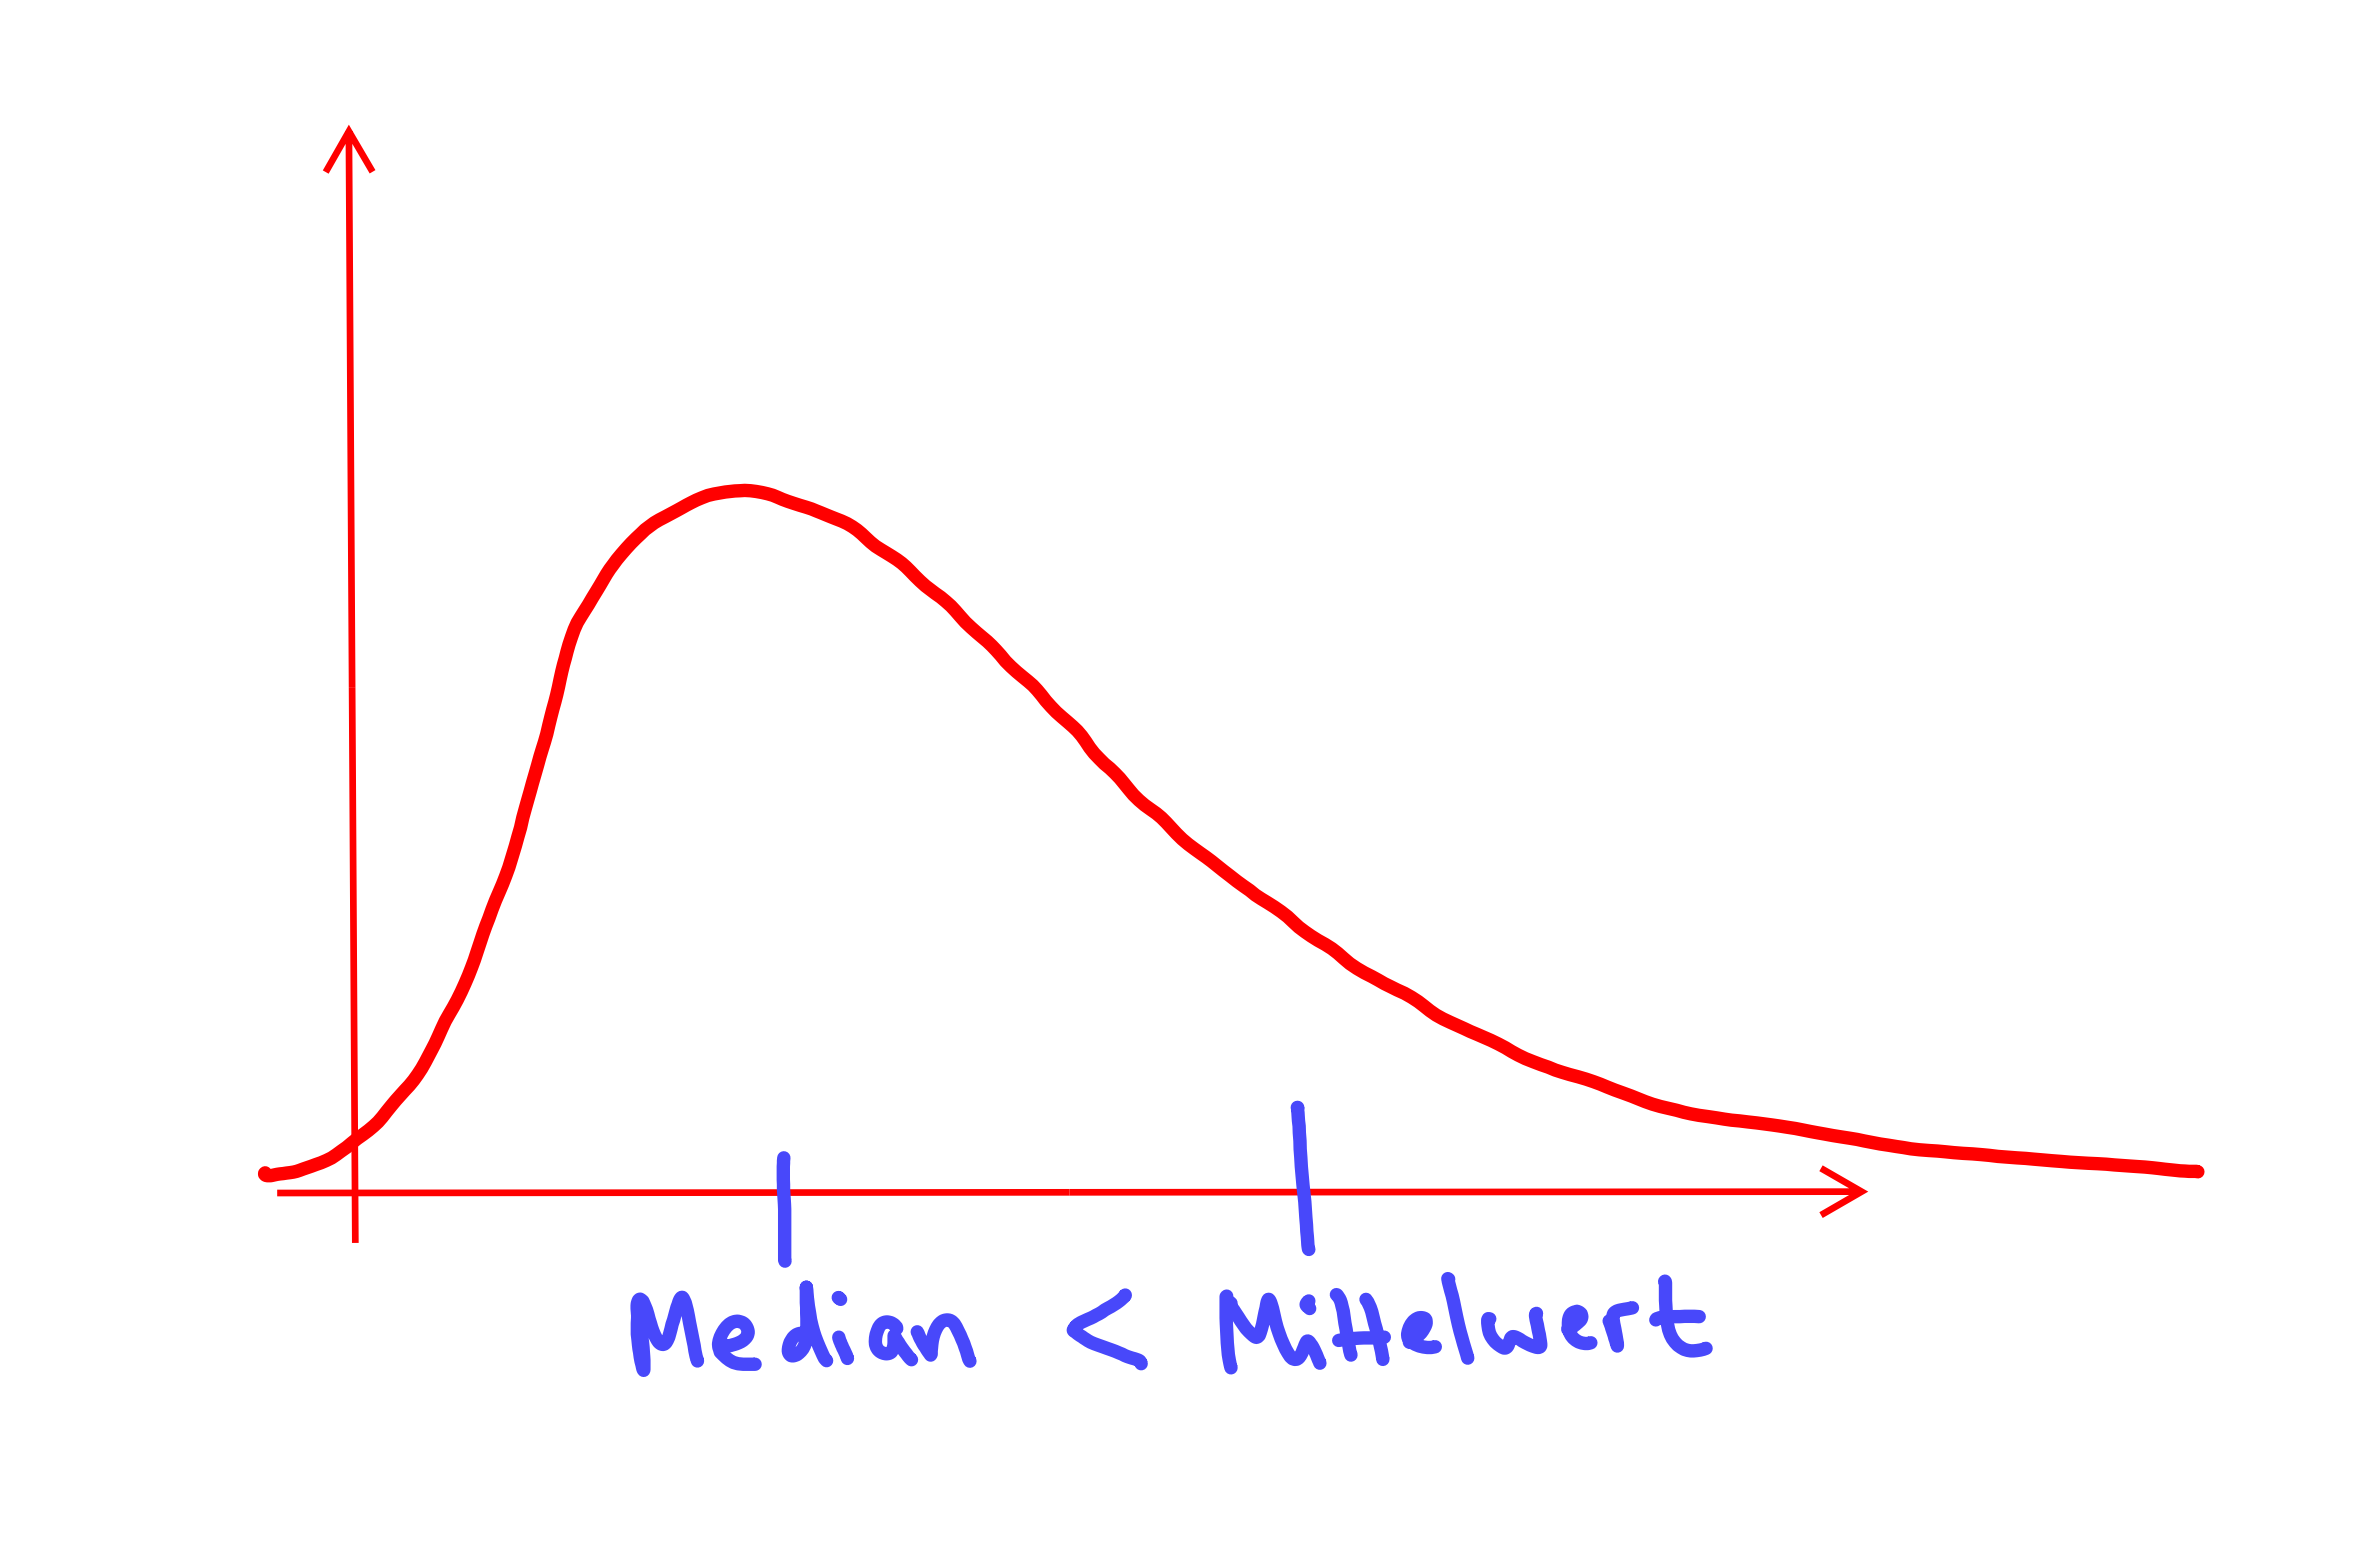
\includegraphics[scale=0.15]{1.png} & 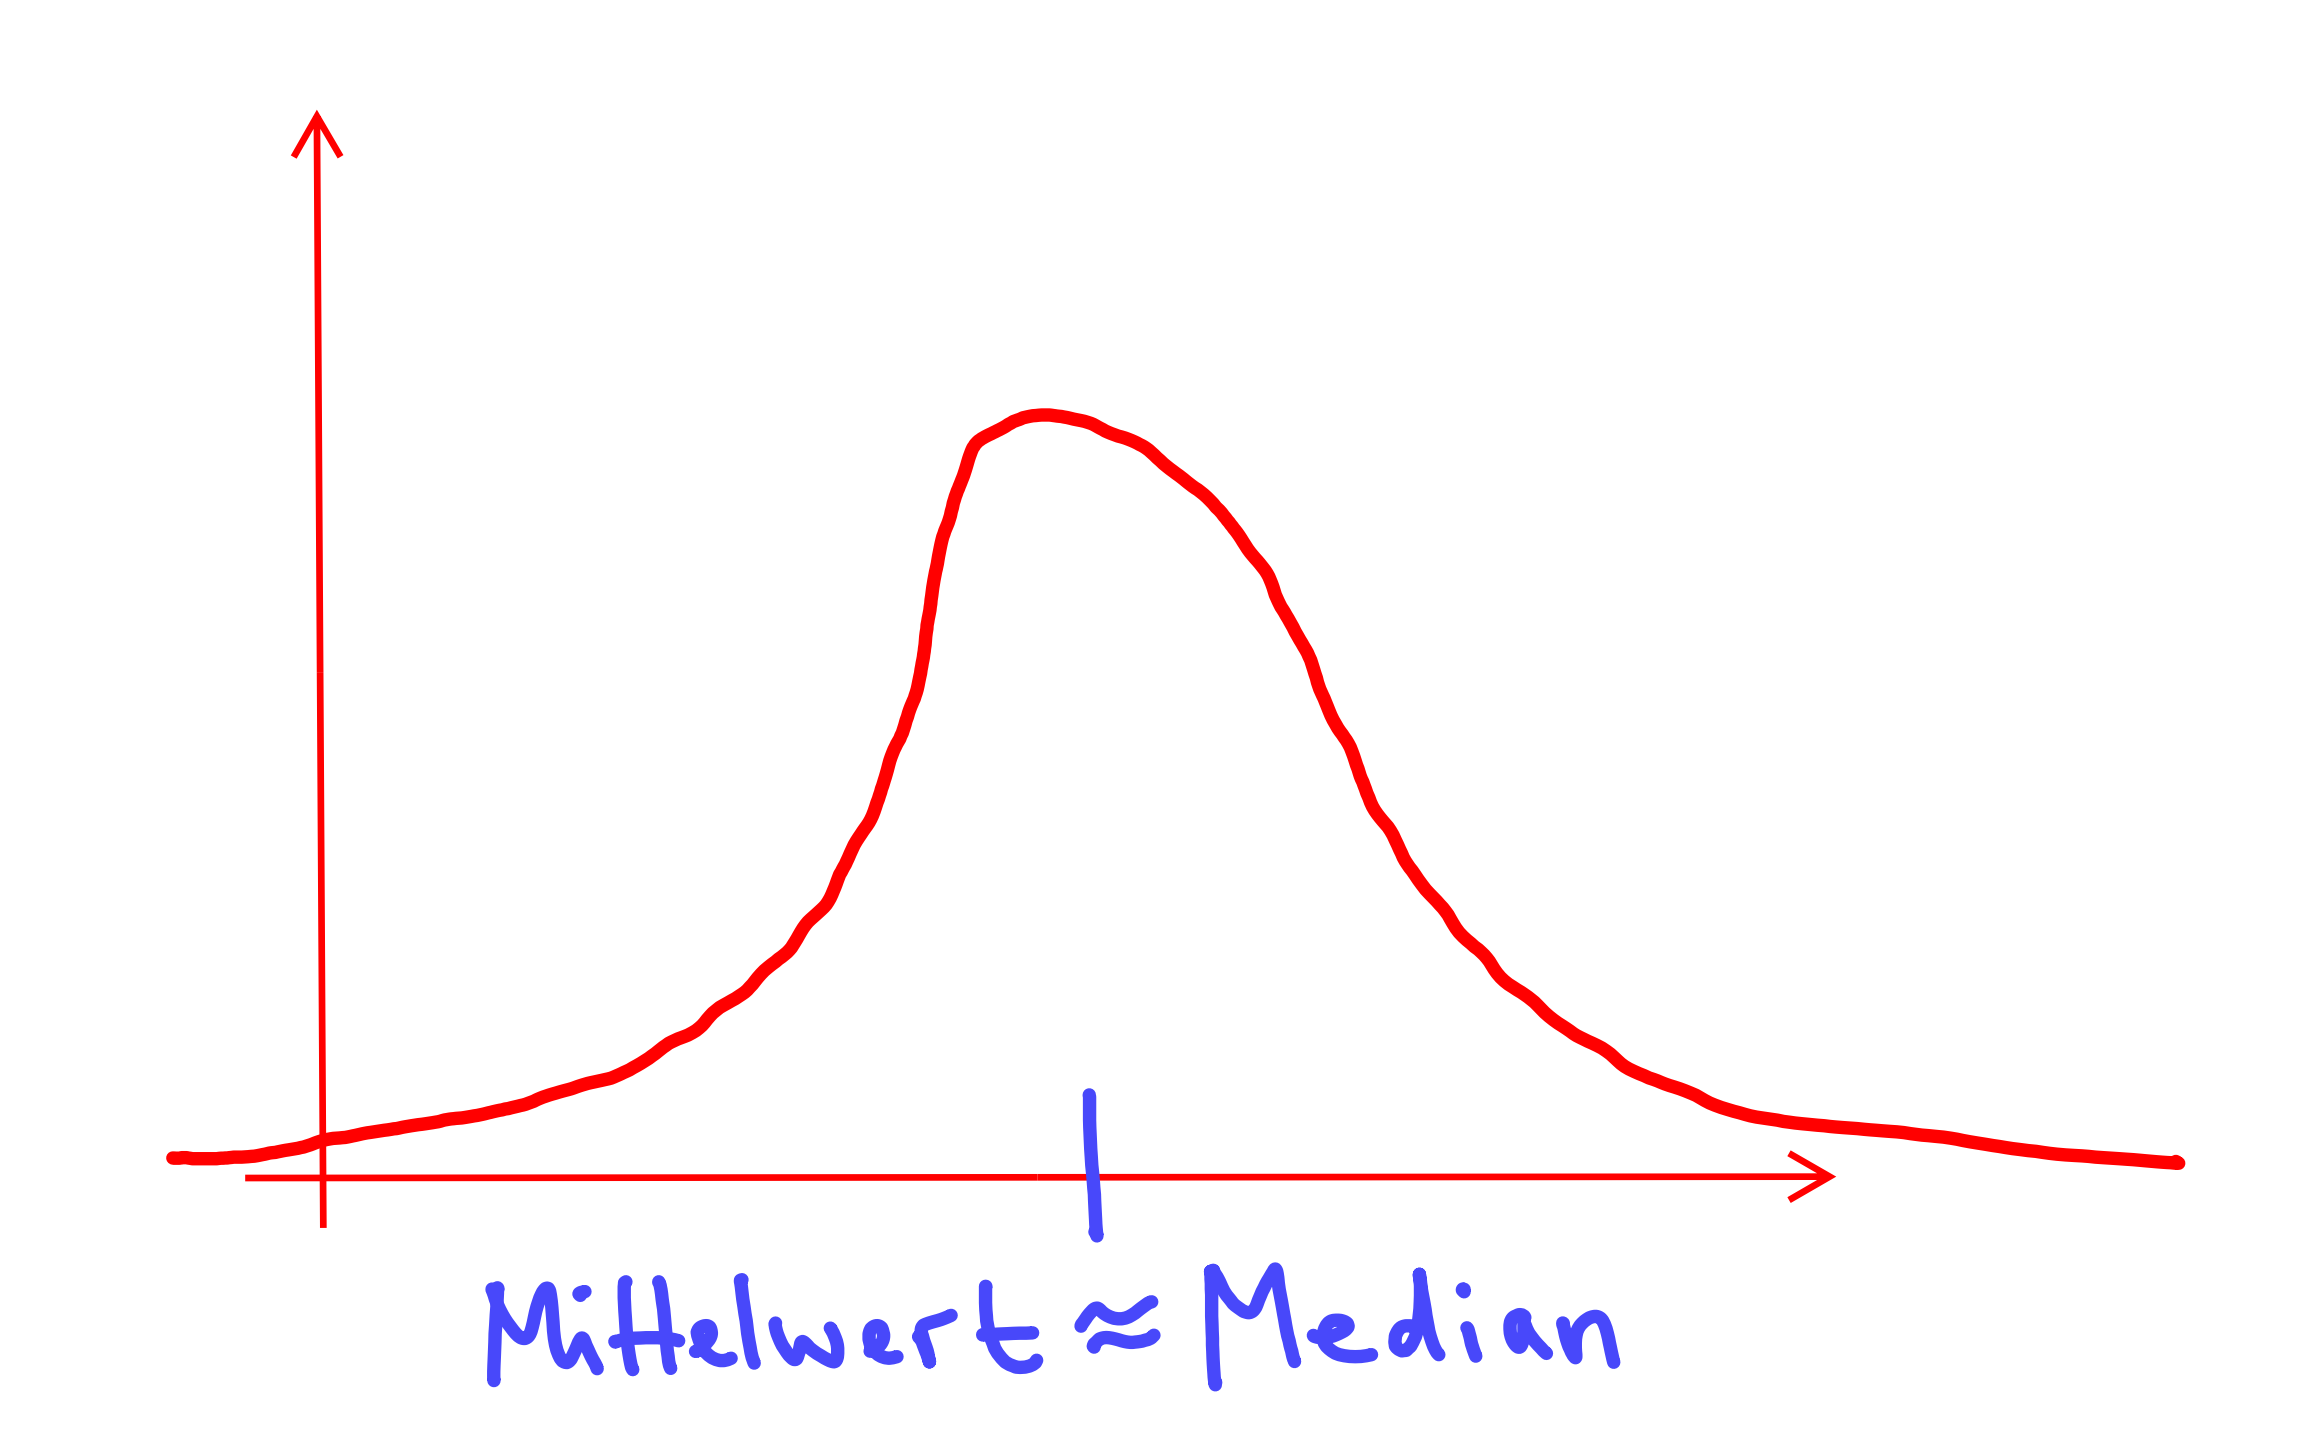
\includegraphics[scale=0.15]{2.png} & 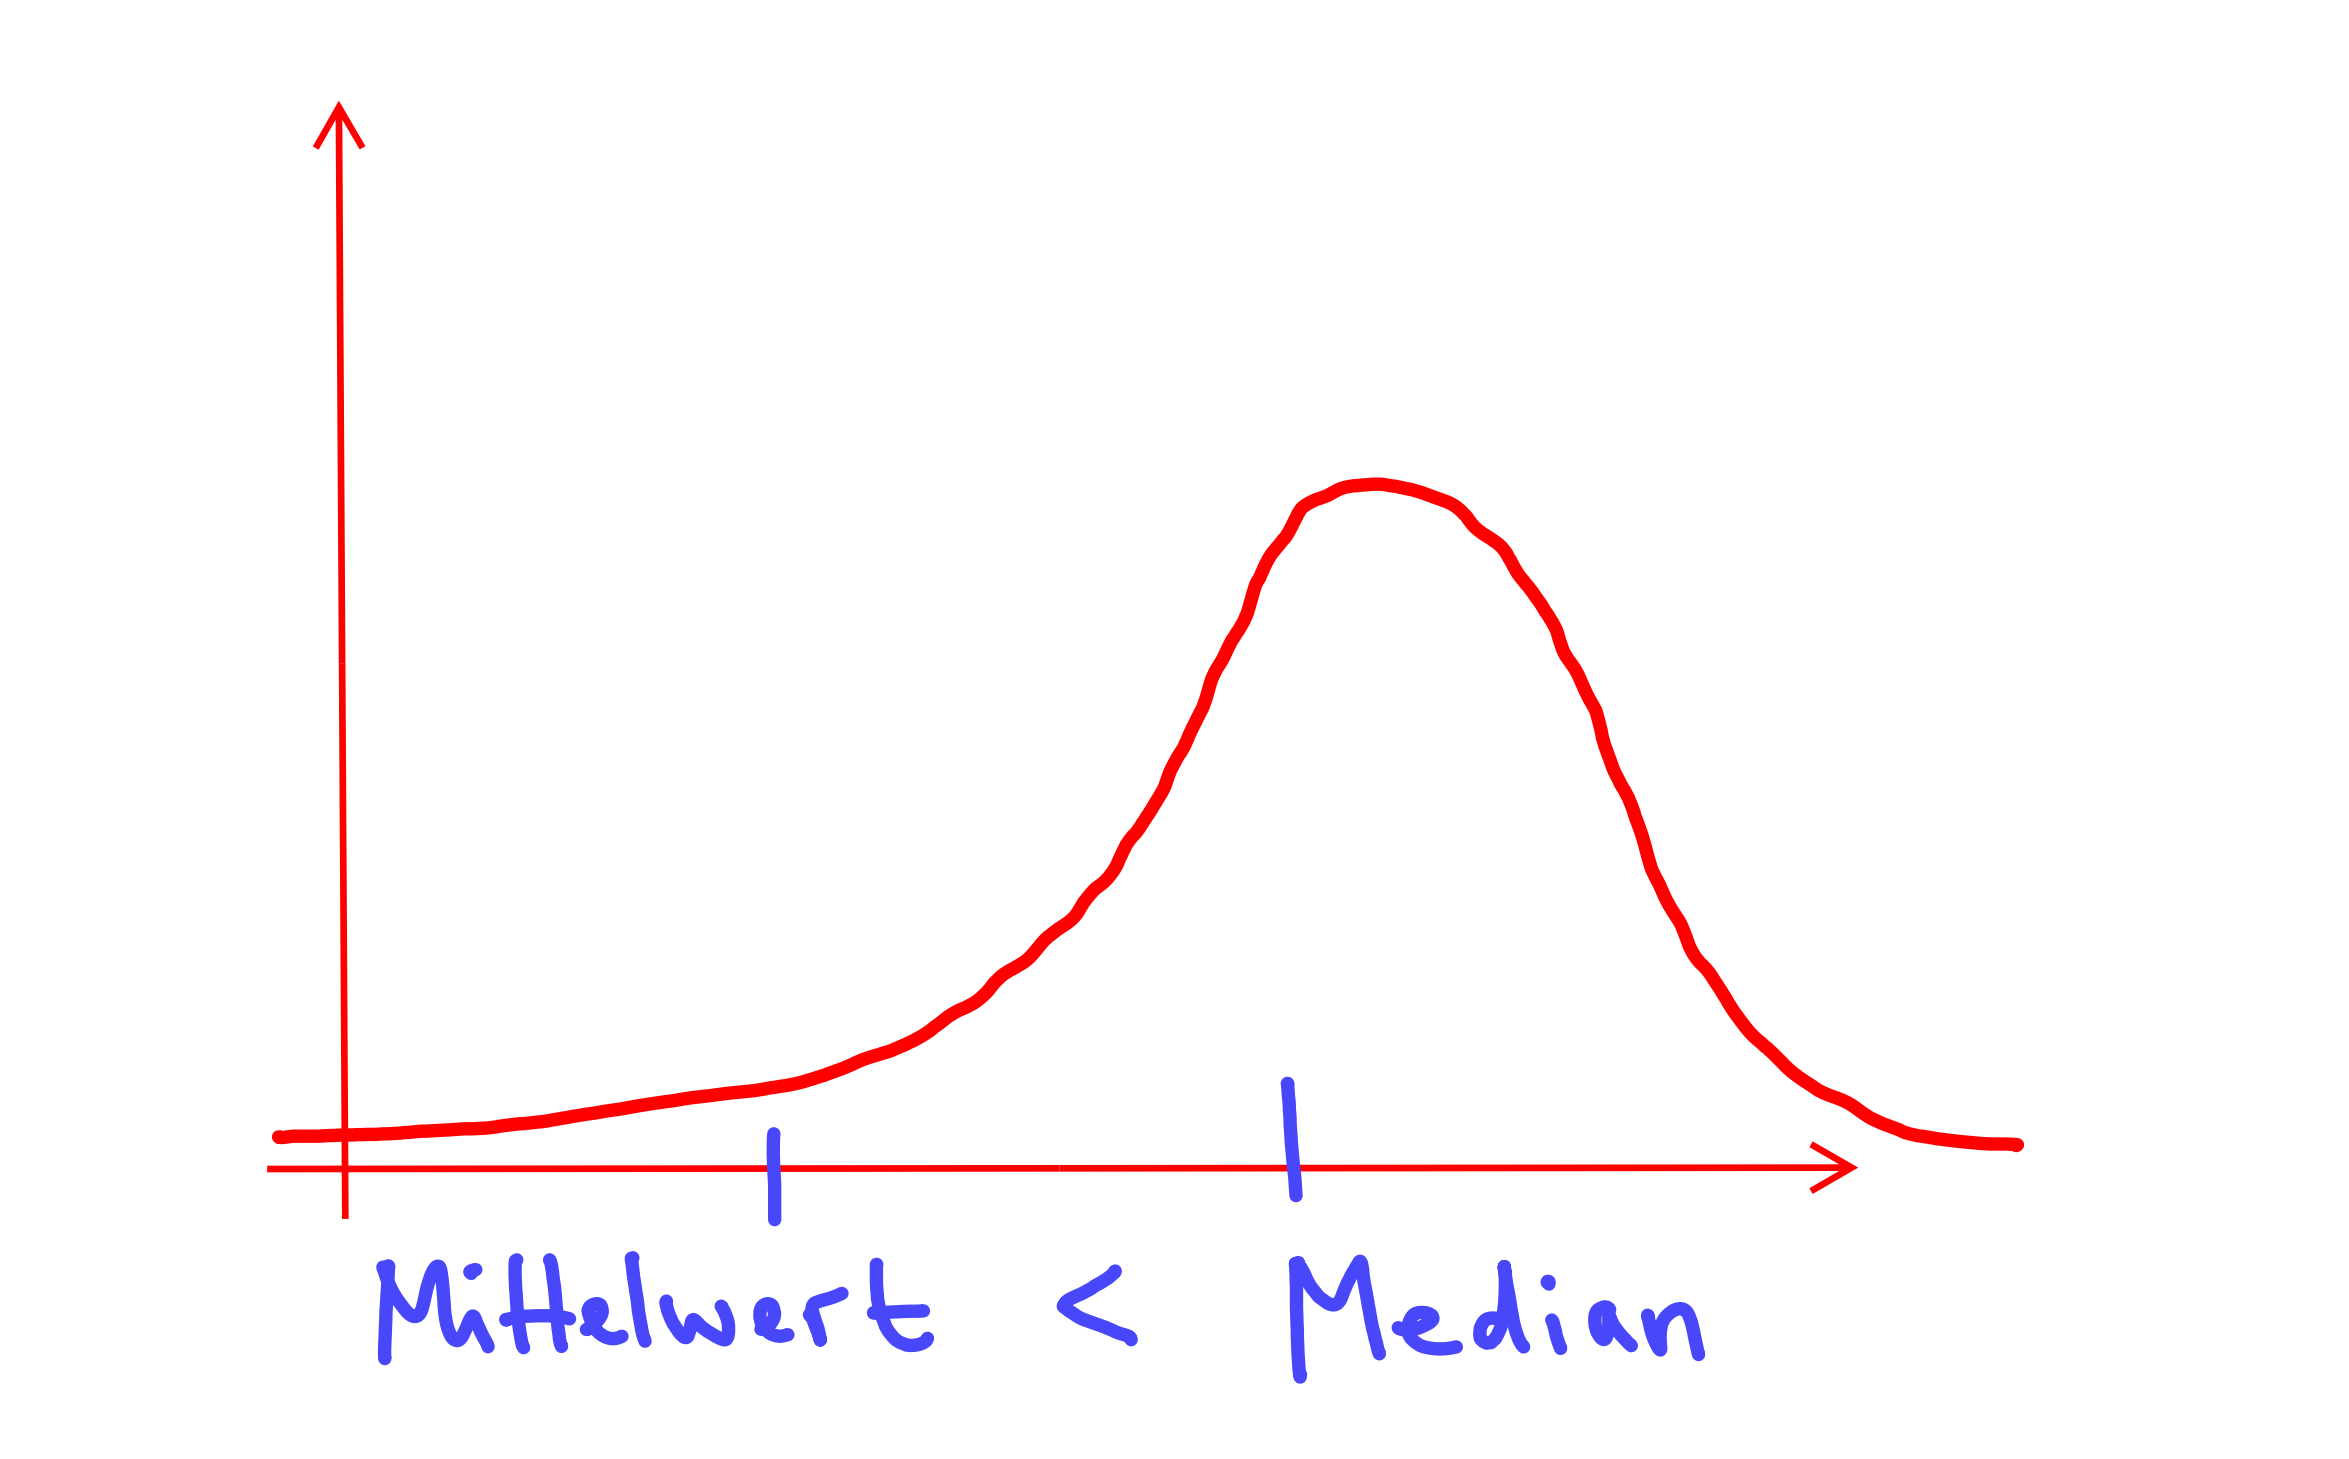
\includegraphics[scale=0.15]{3.png}  
		\end{tabular} 
	\end{center}
\end{frame}

\begin{frame}
	Der Mittelwert ist ausreißerempfindlich, der Median nicht!
	\begin{center}
		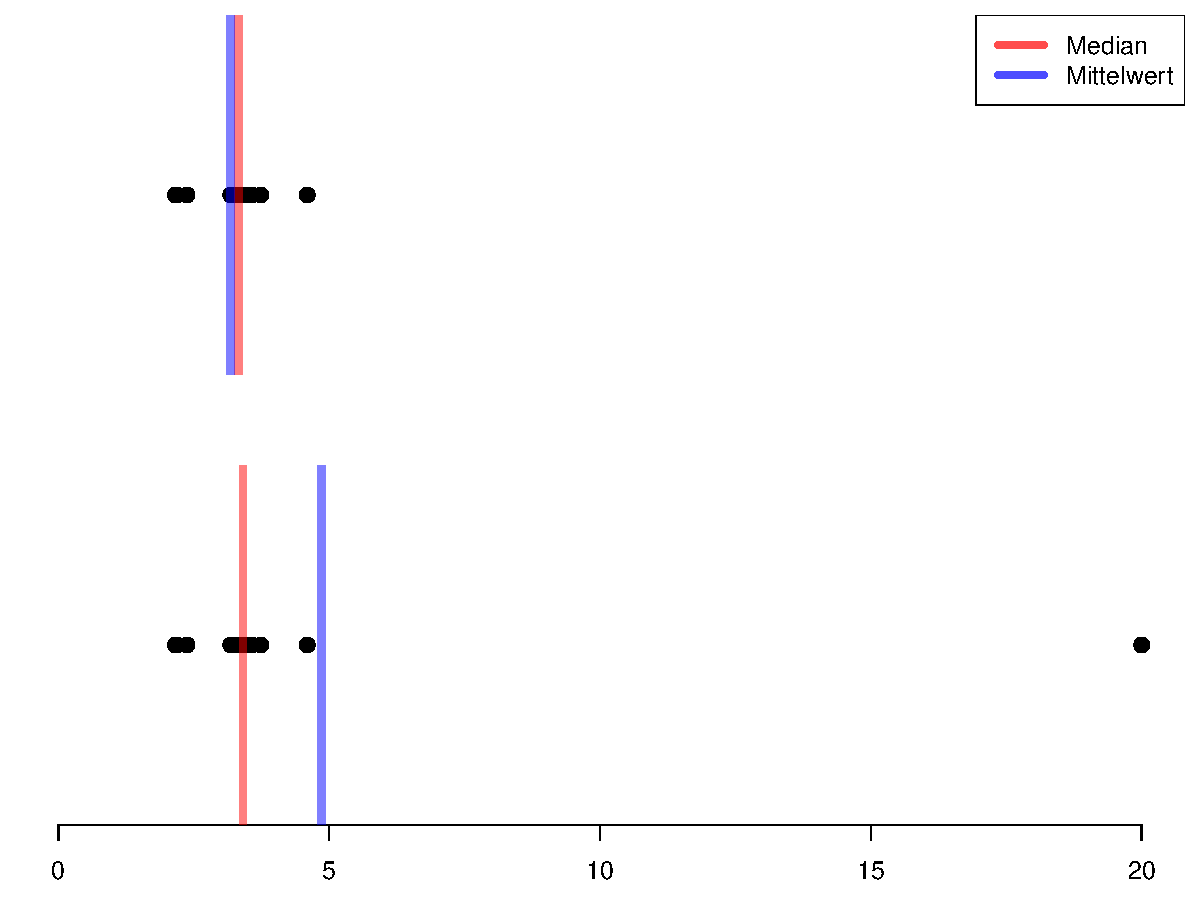
\includegraphics[scale=0.4]{outlier.pdf}
	\end{center}
\end{frame}

\begin{frame}
Schiefetypen
\begin{center}
	\begin{tabular}{ccc}
		linkssteil / rechtsschief & symmetrisch & rechtssteil / linksschief  \\
		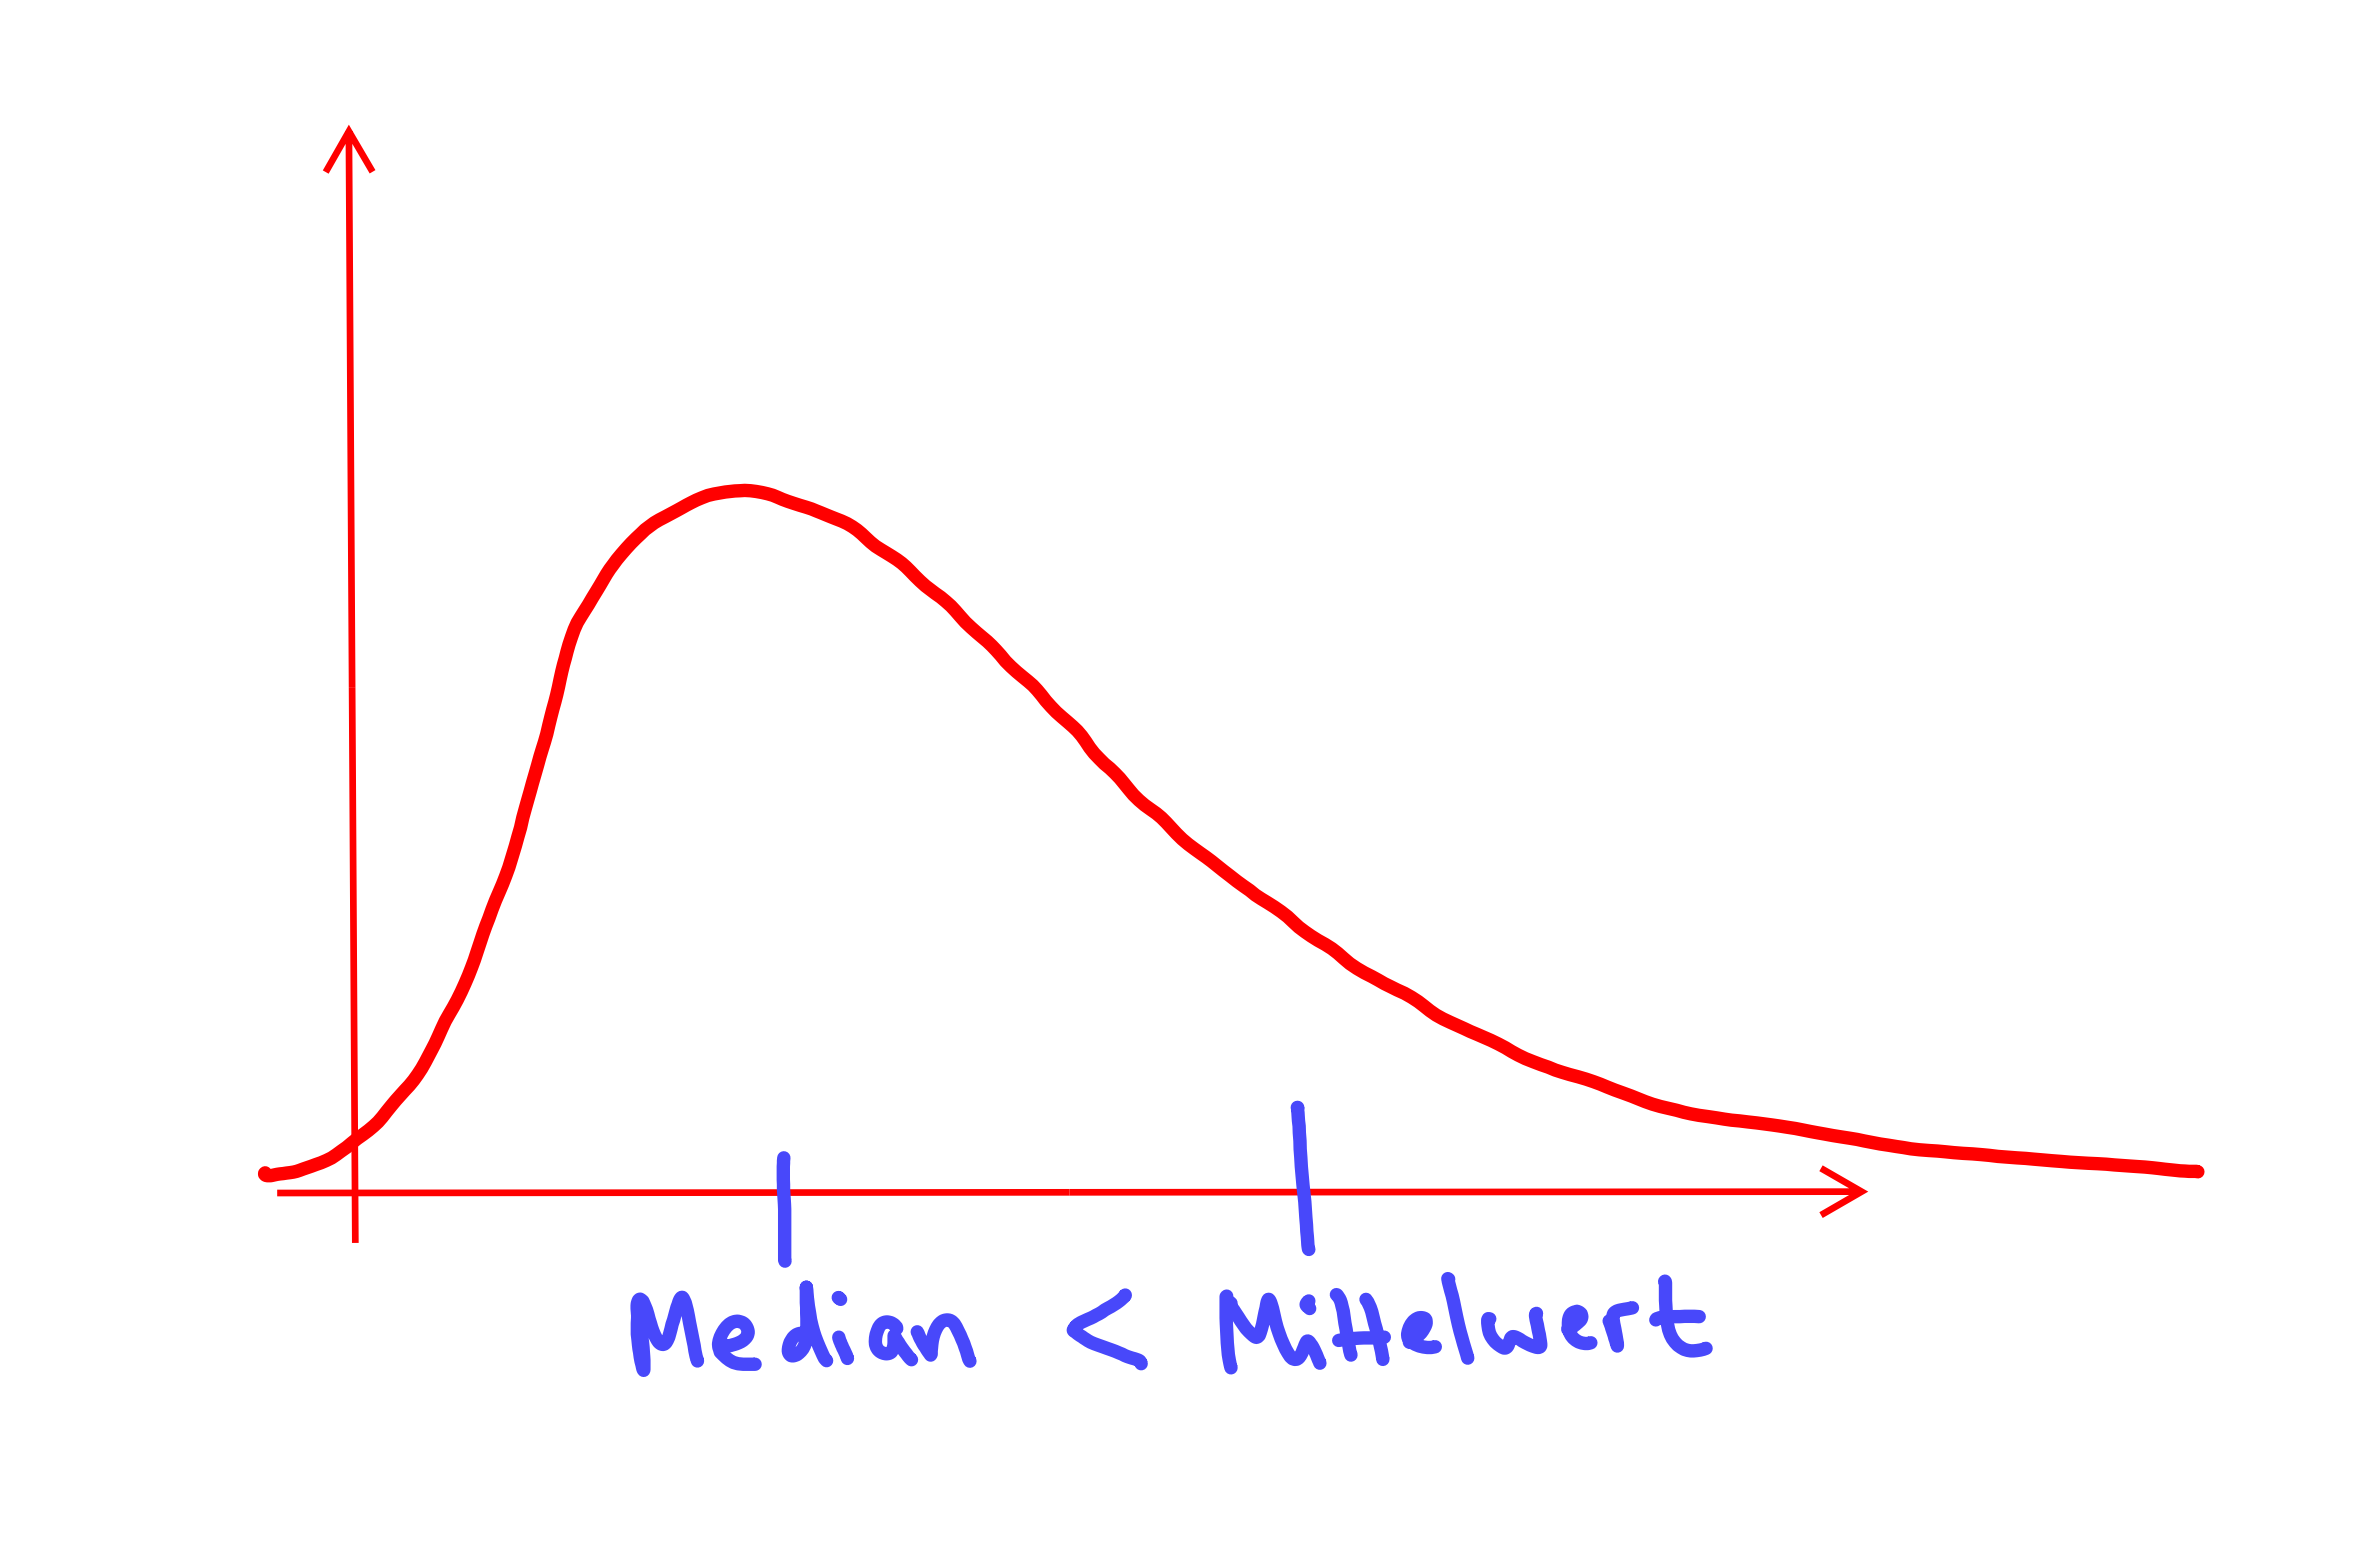
\includegraphics[scale=0.15]{1.png} & 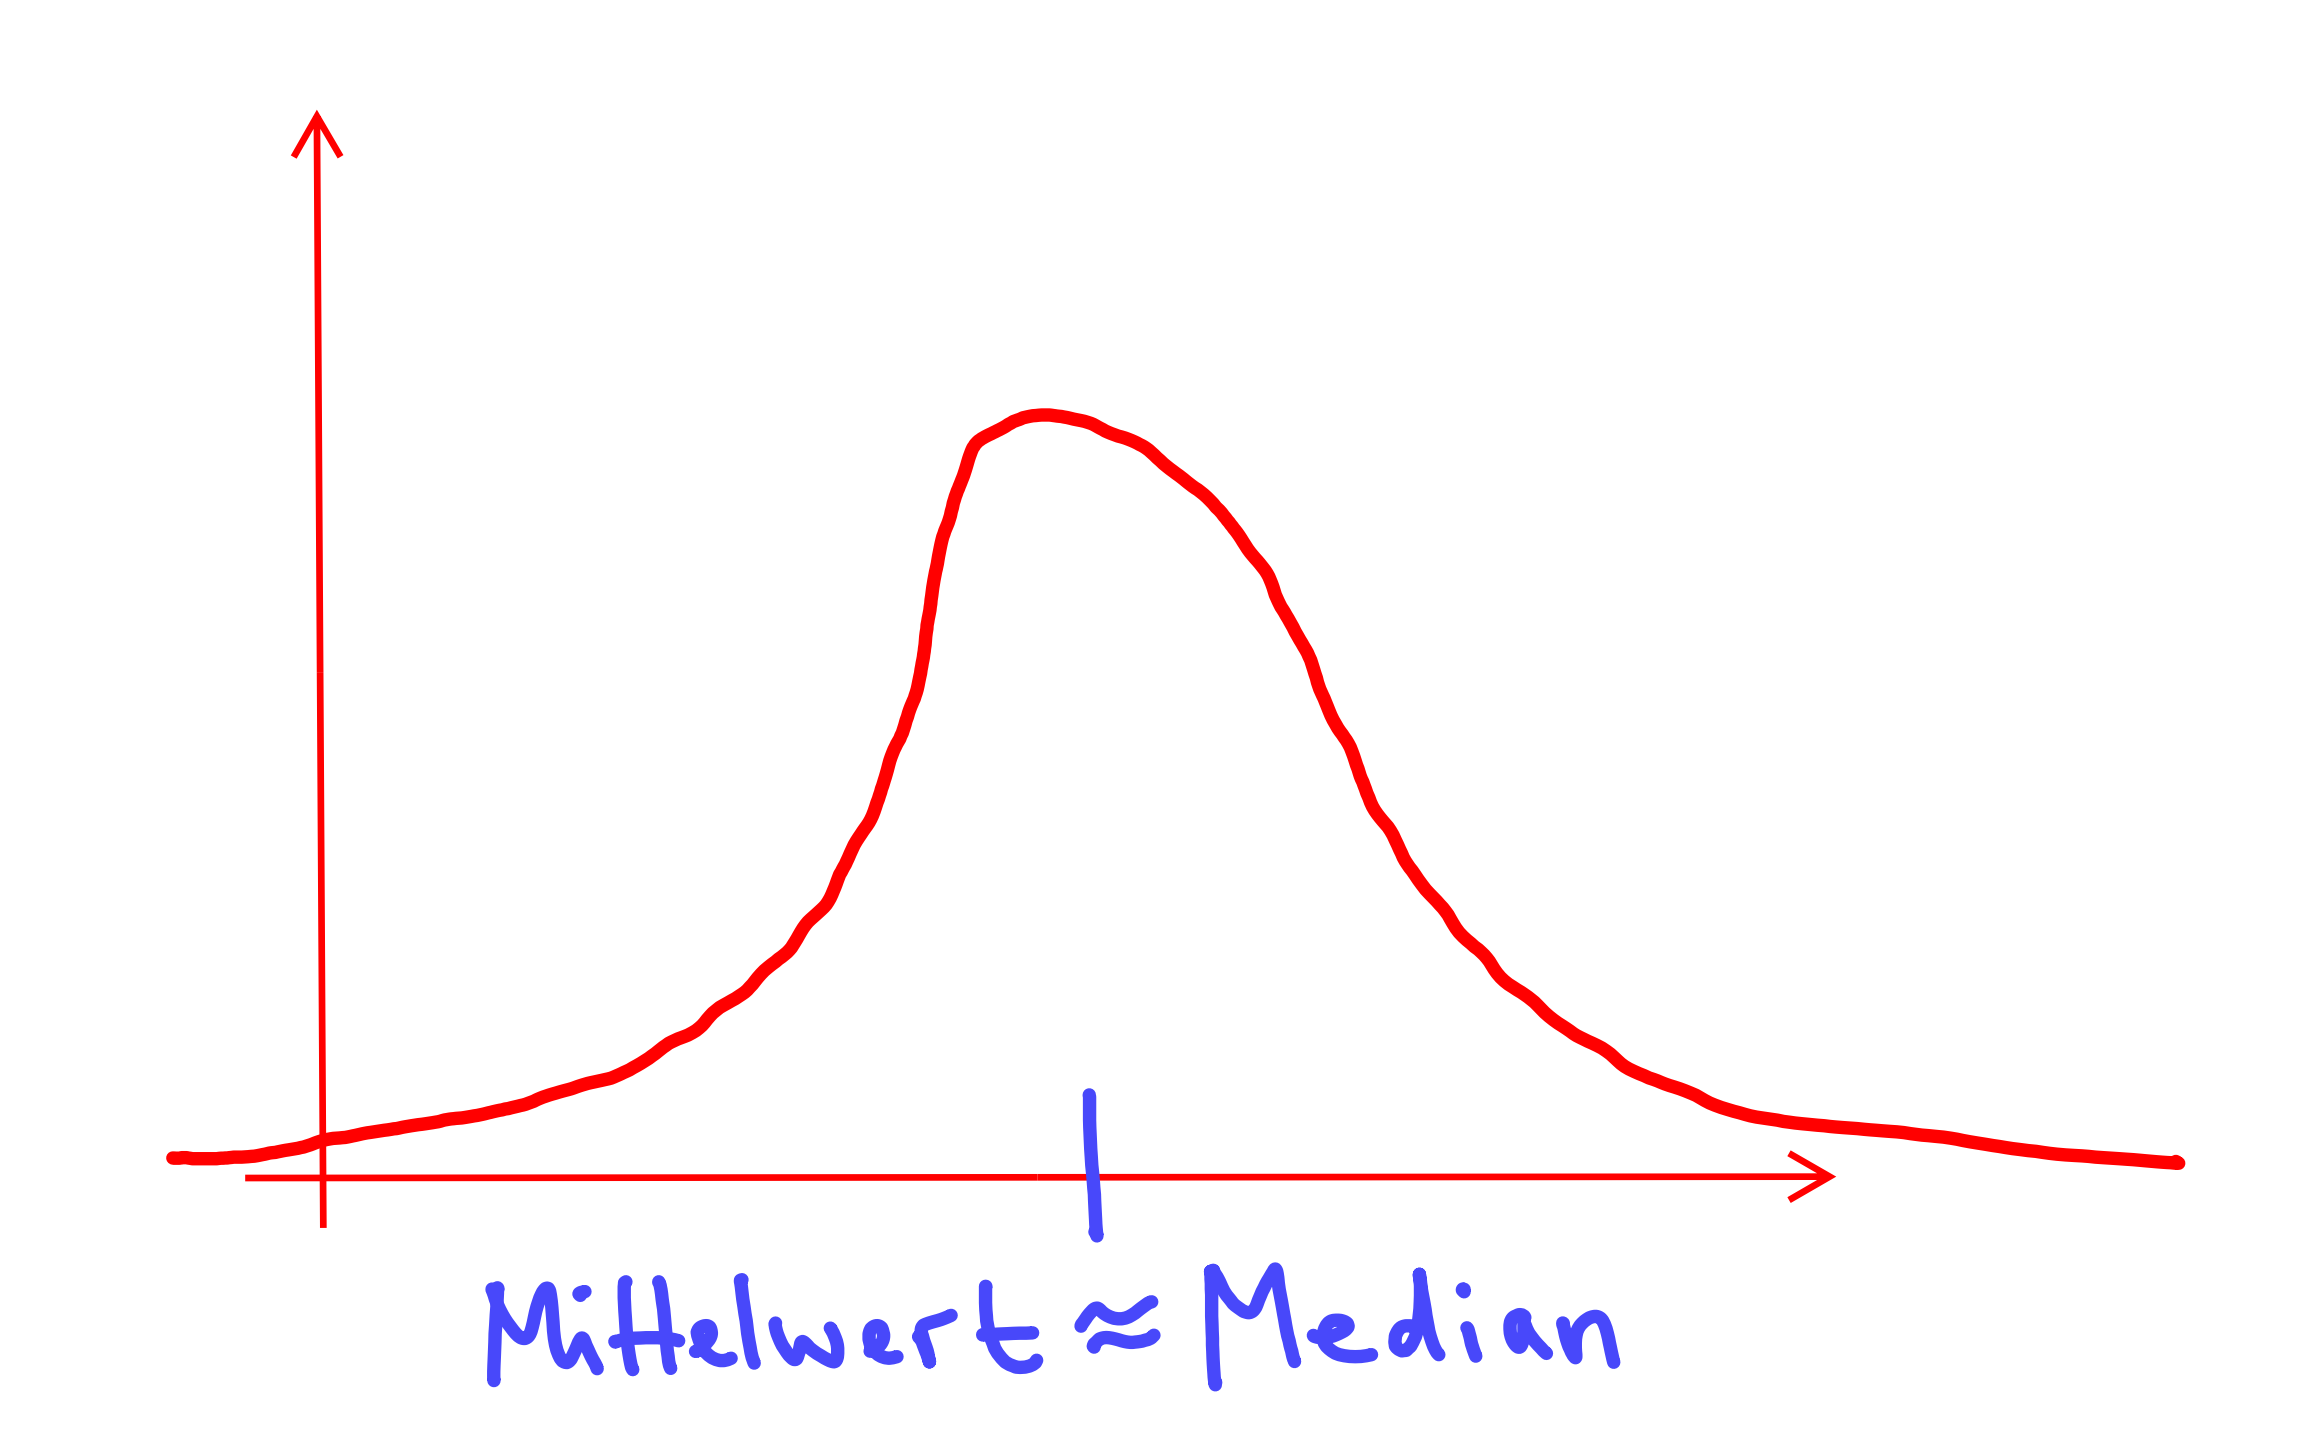
\includegraphics[scale=0.15]{2.png} & 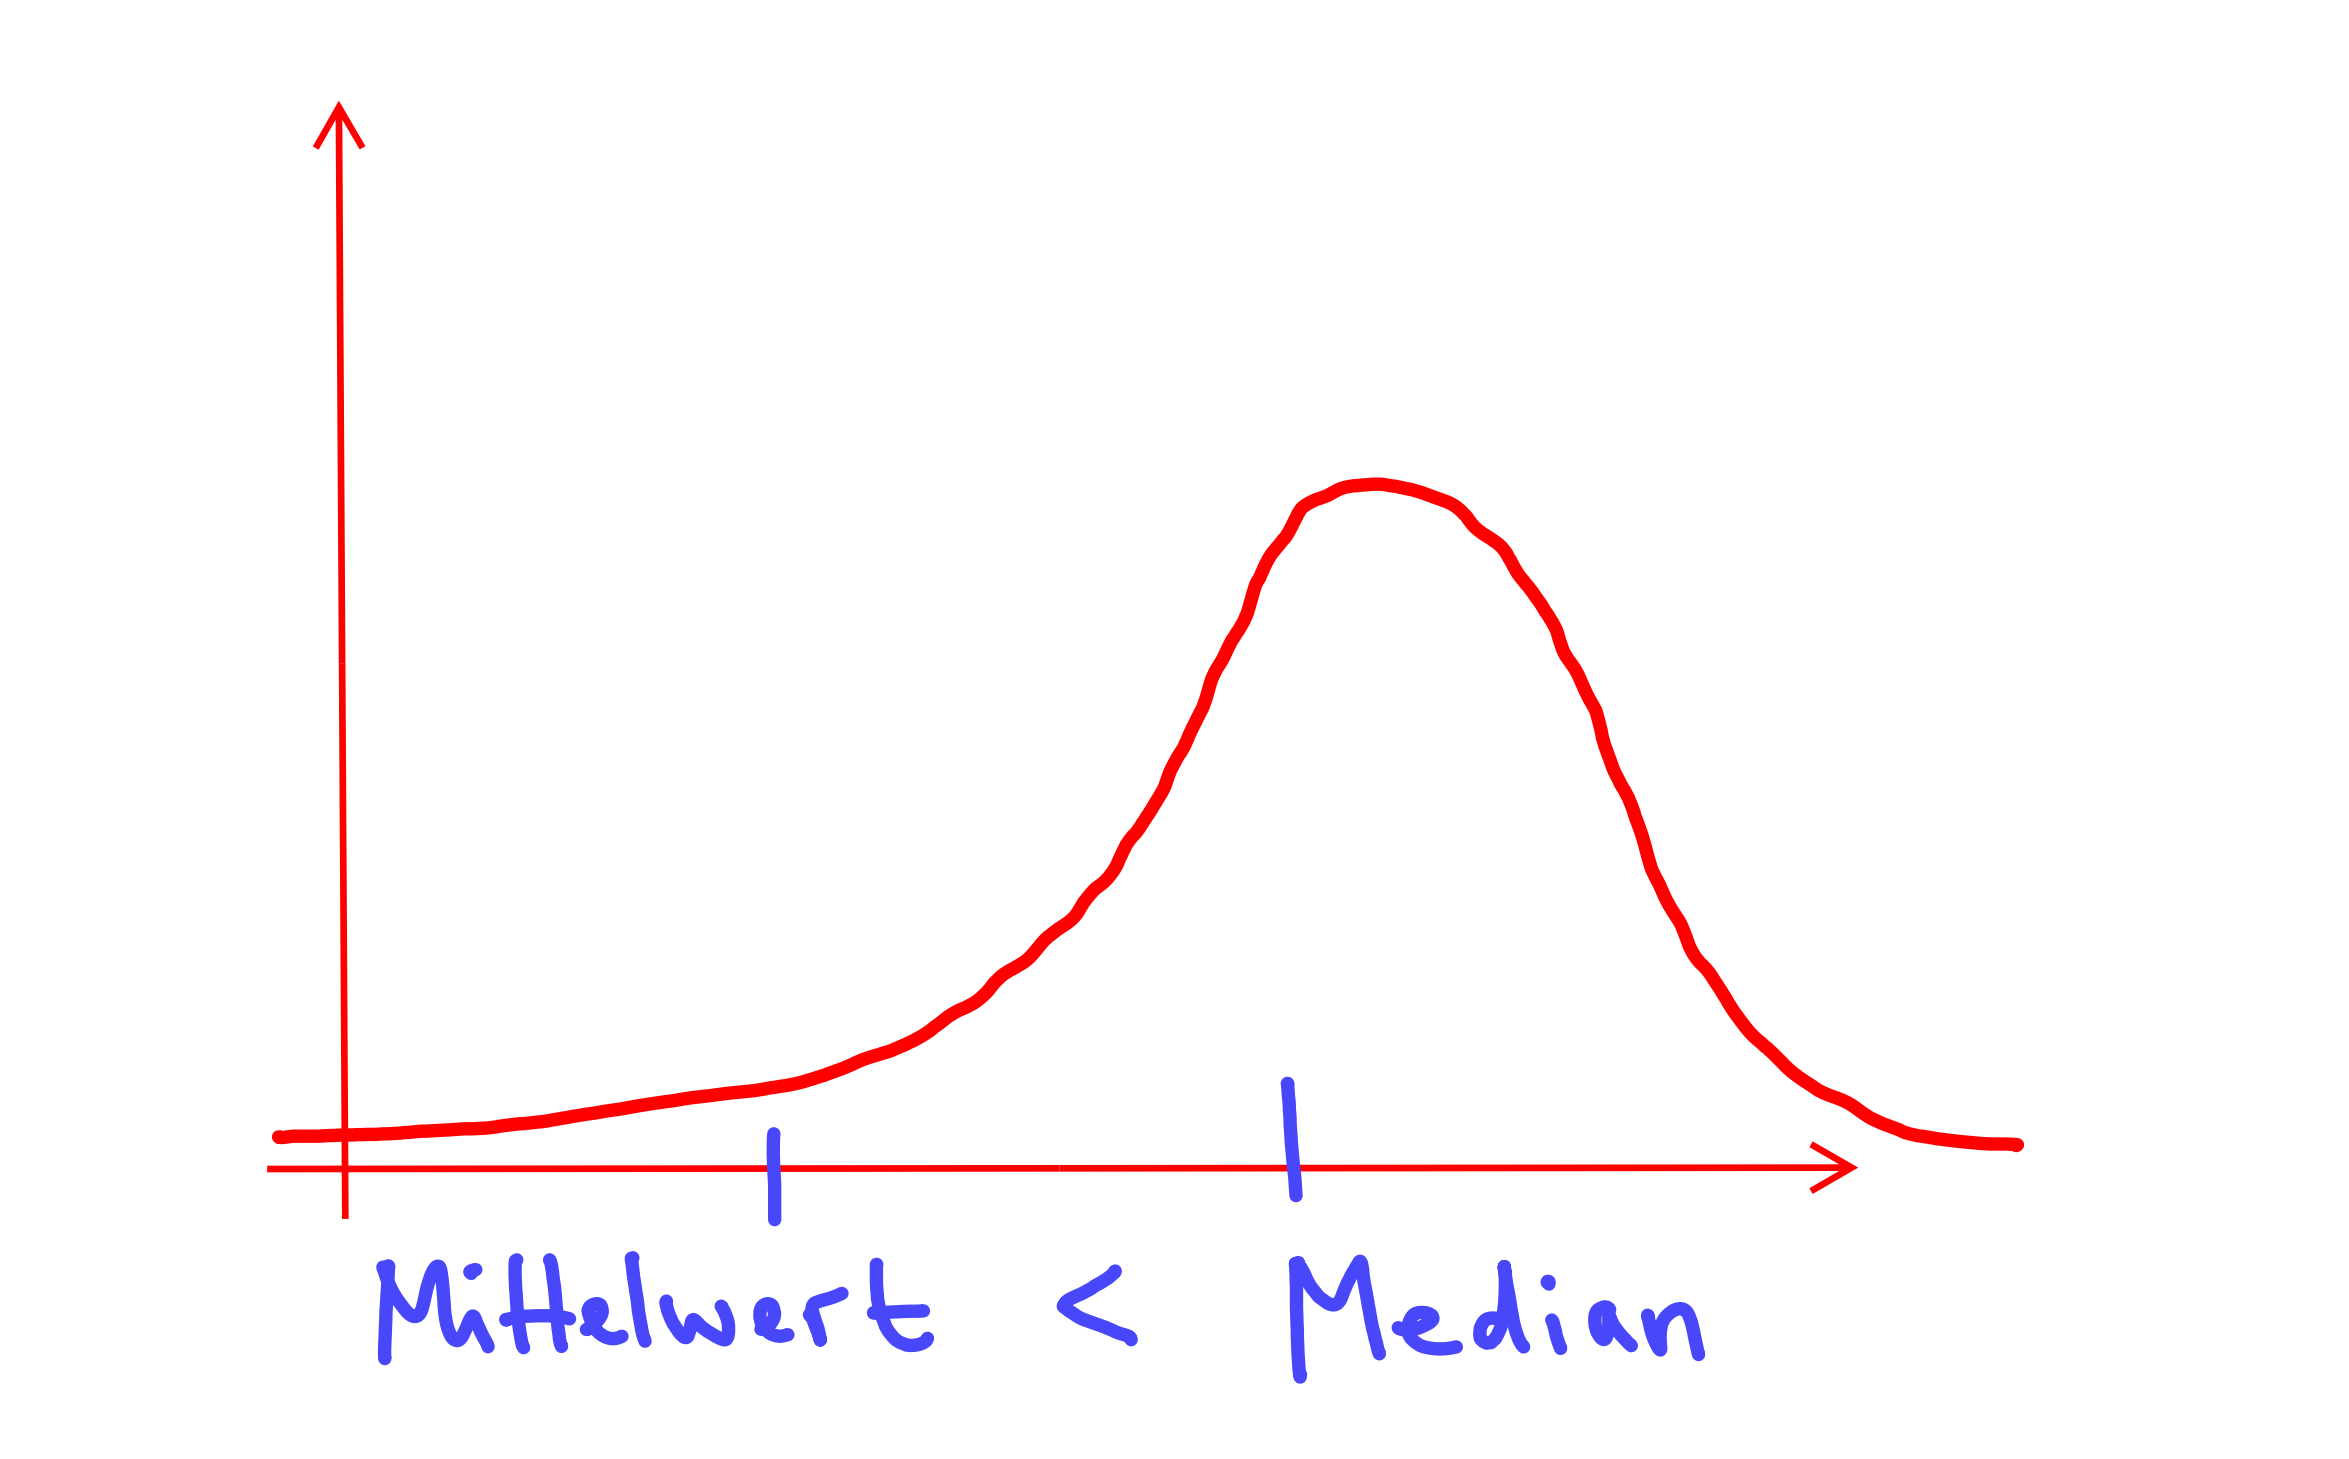
\includegraphics[scale=0.15]{3.png}  
	\end{tabular} 
\end{center}
\end{frame}

\begin{frame}
Schiefetypen
\begin{center}
	\begin{tabular}{ccc}
		linkssteil / rechtsschief & symmetrisch & rechtssteil / linksschief  \\
		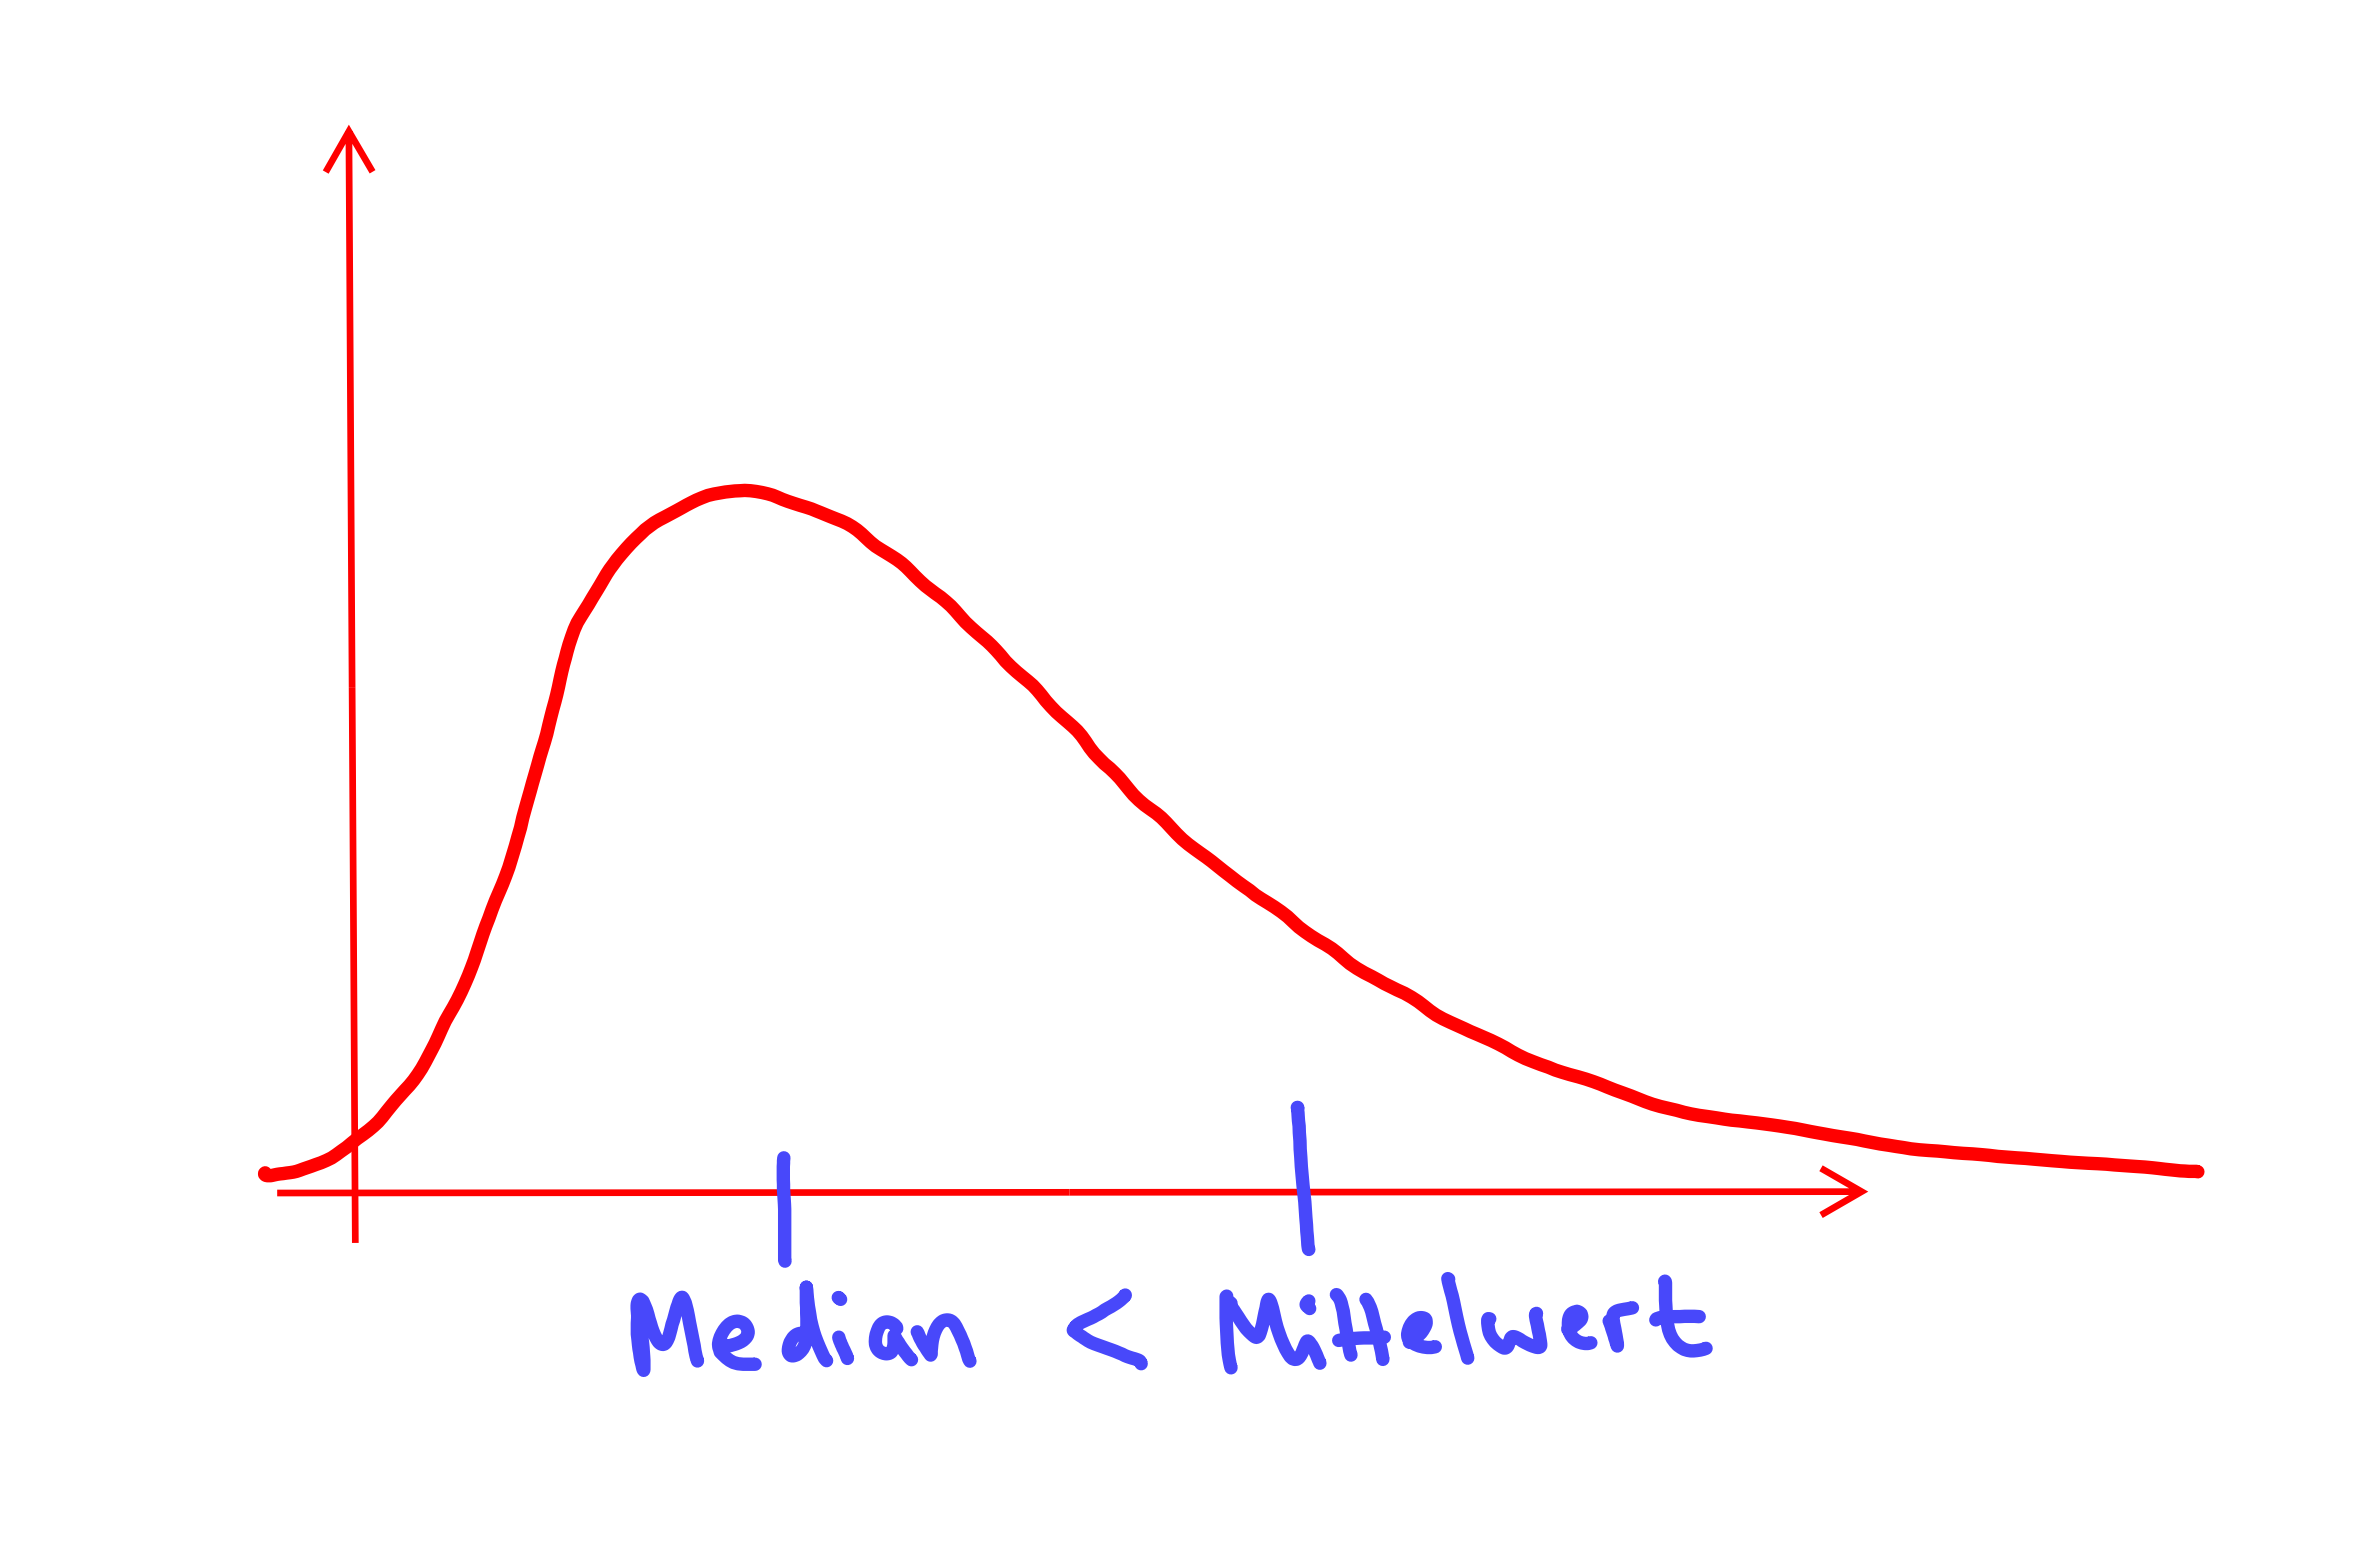
\includegraphics[scale=0.15]{1.png} & 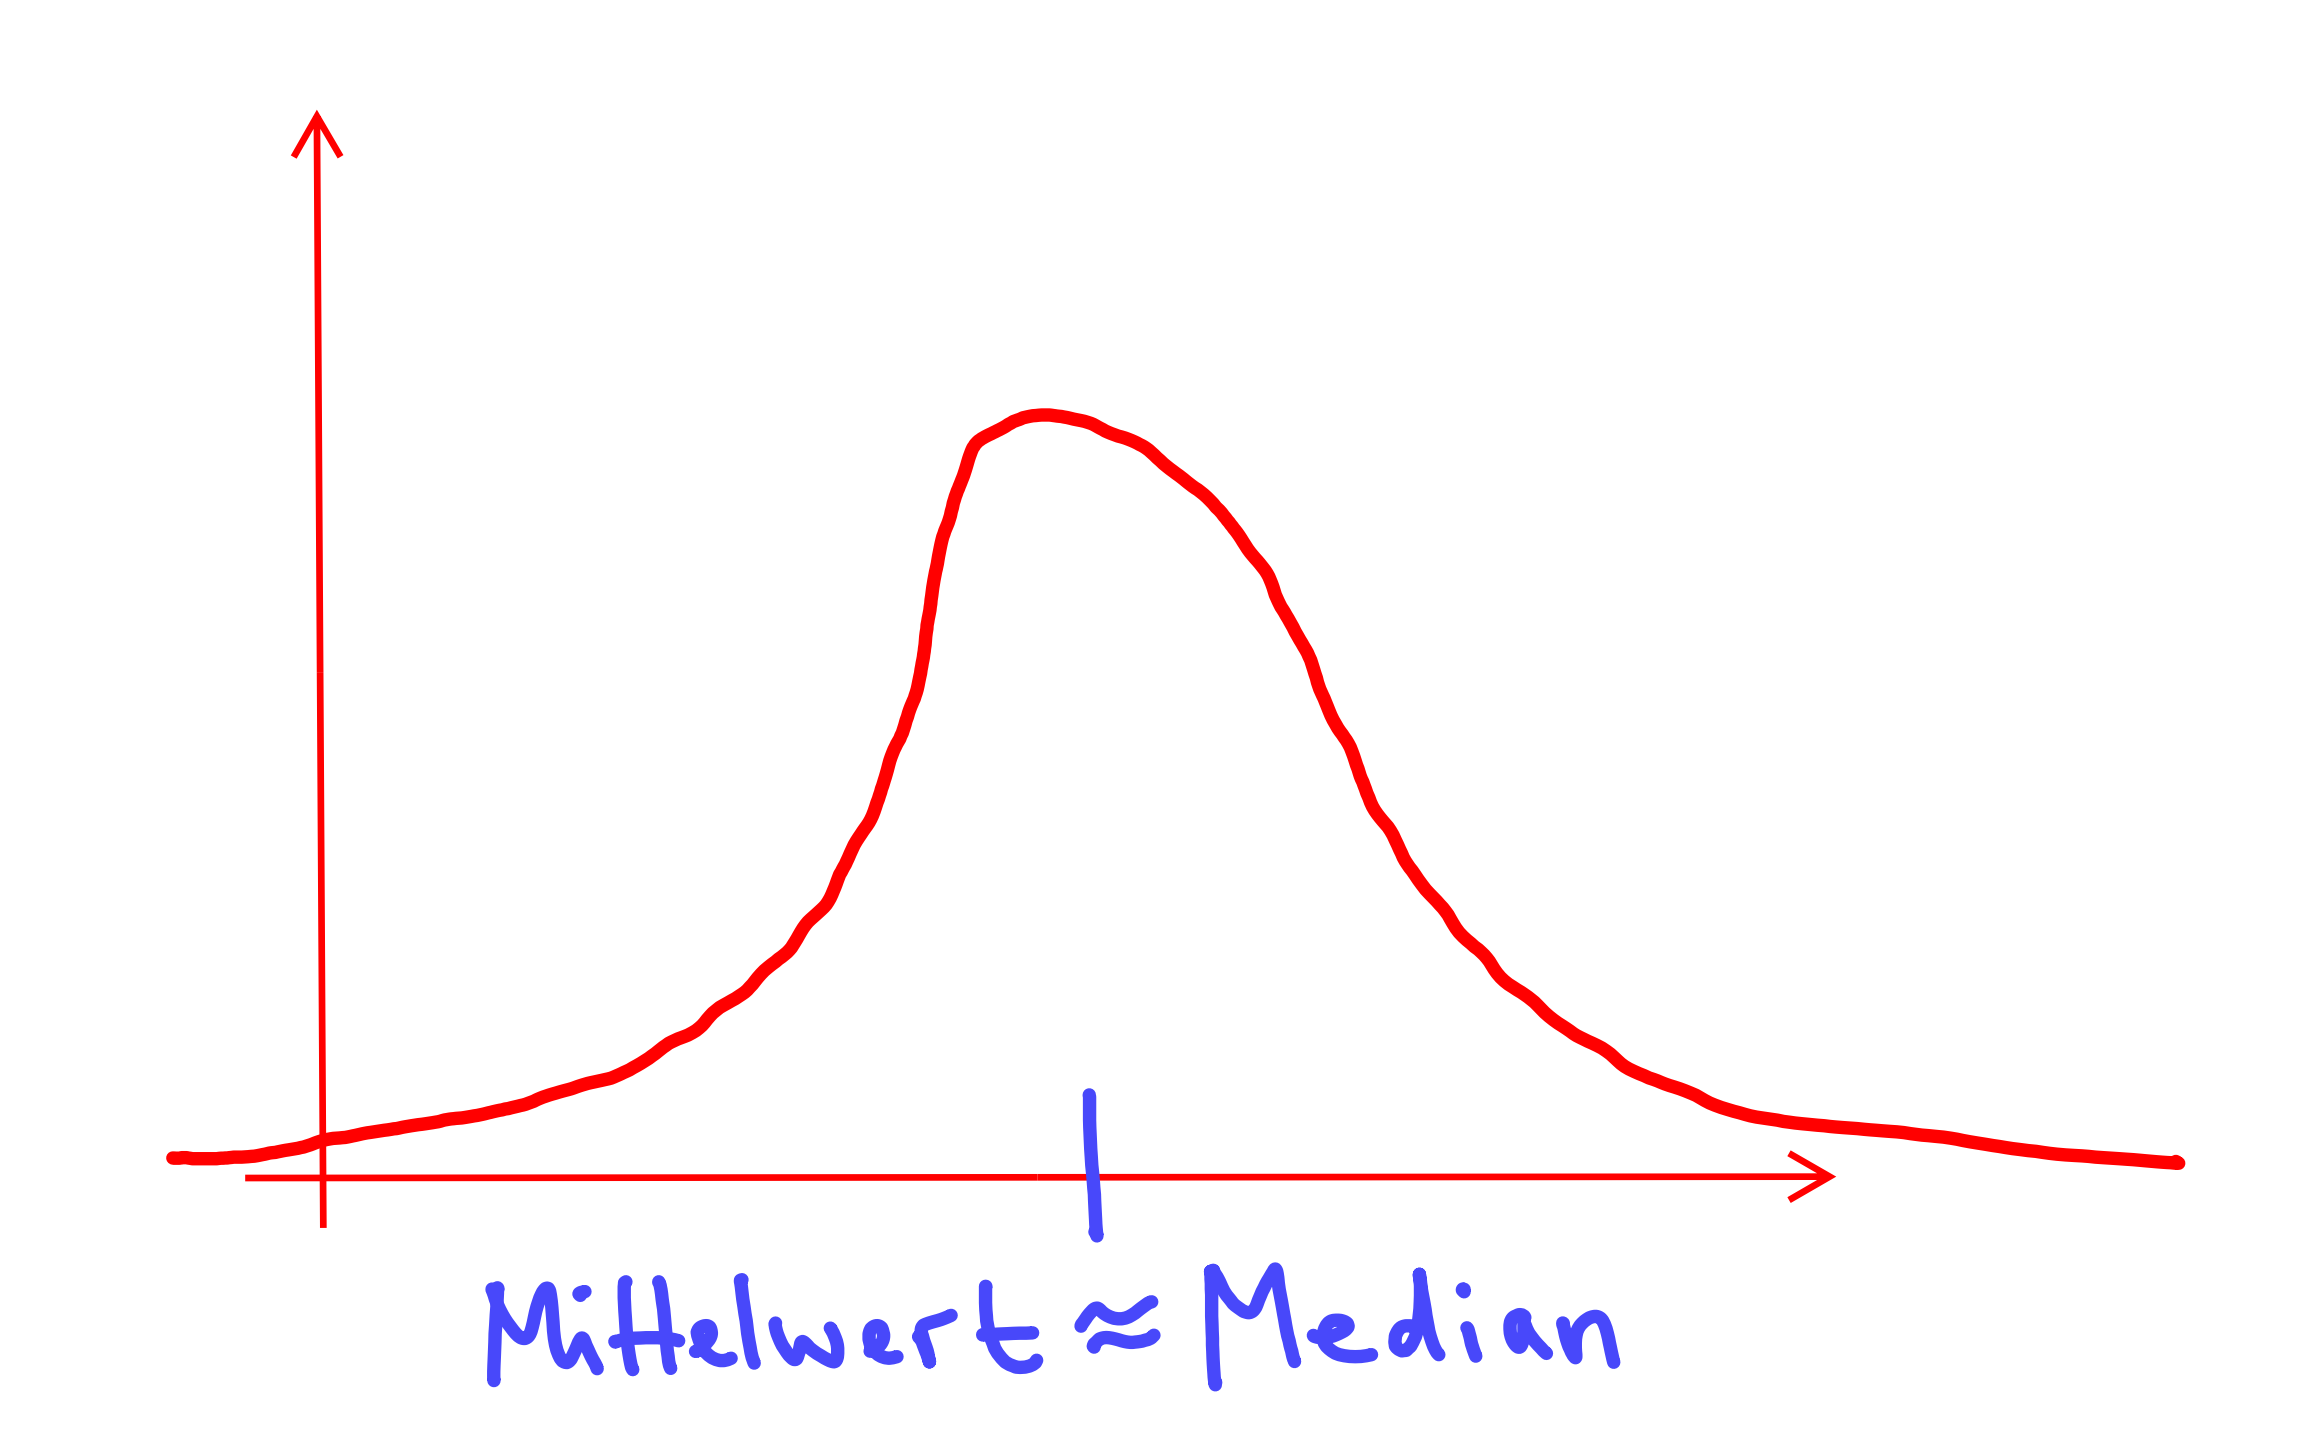
\includegraphics[scale=0.15]{2.png} & 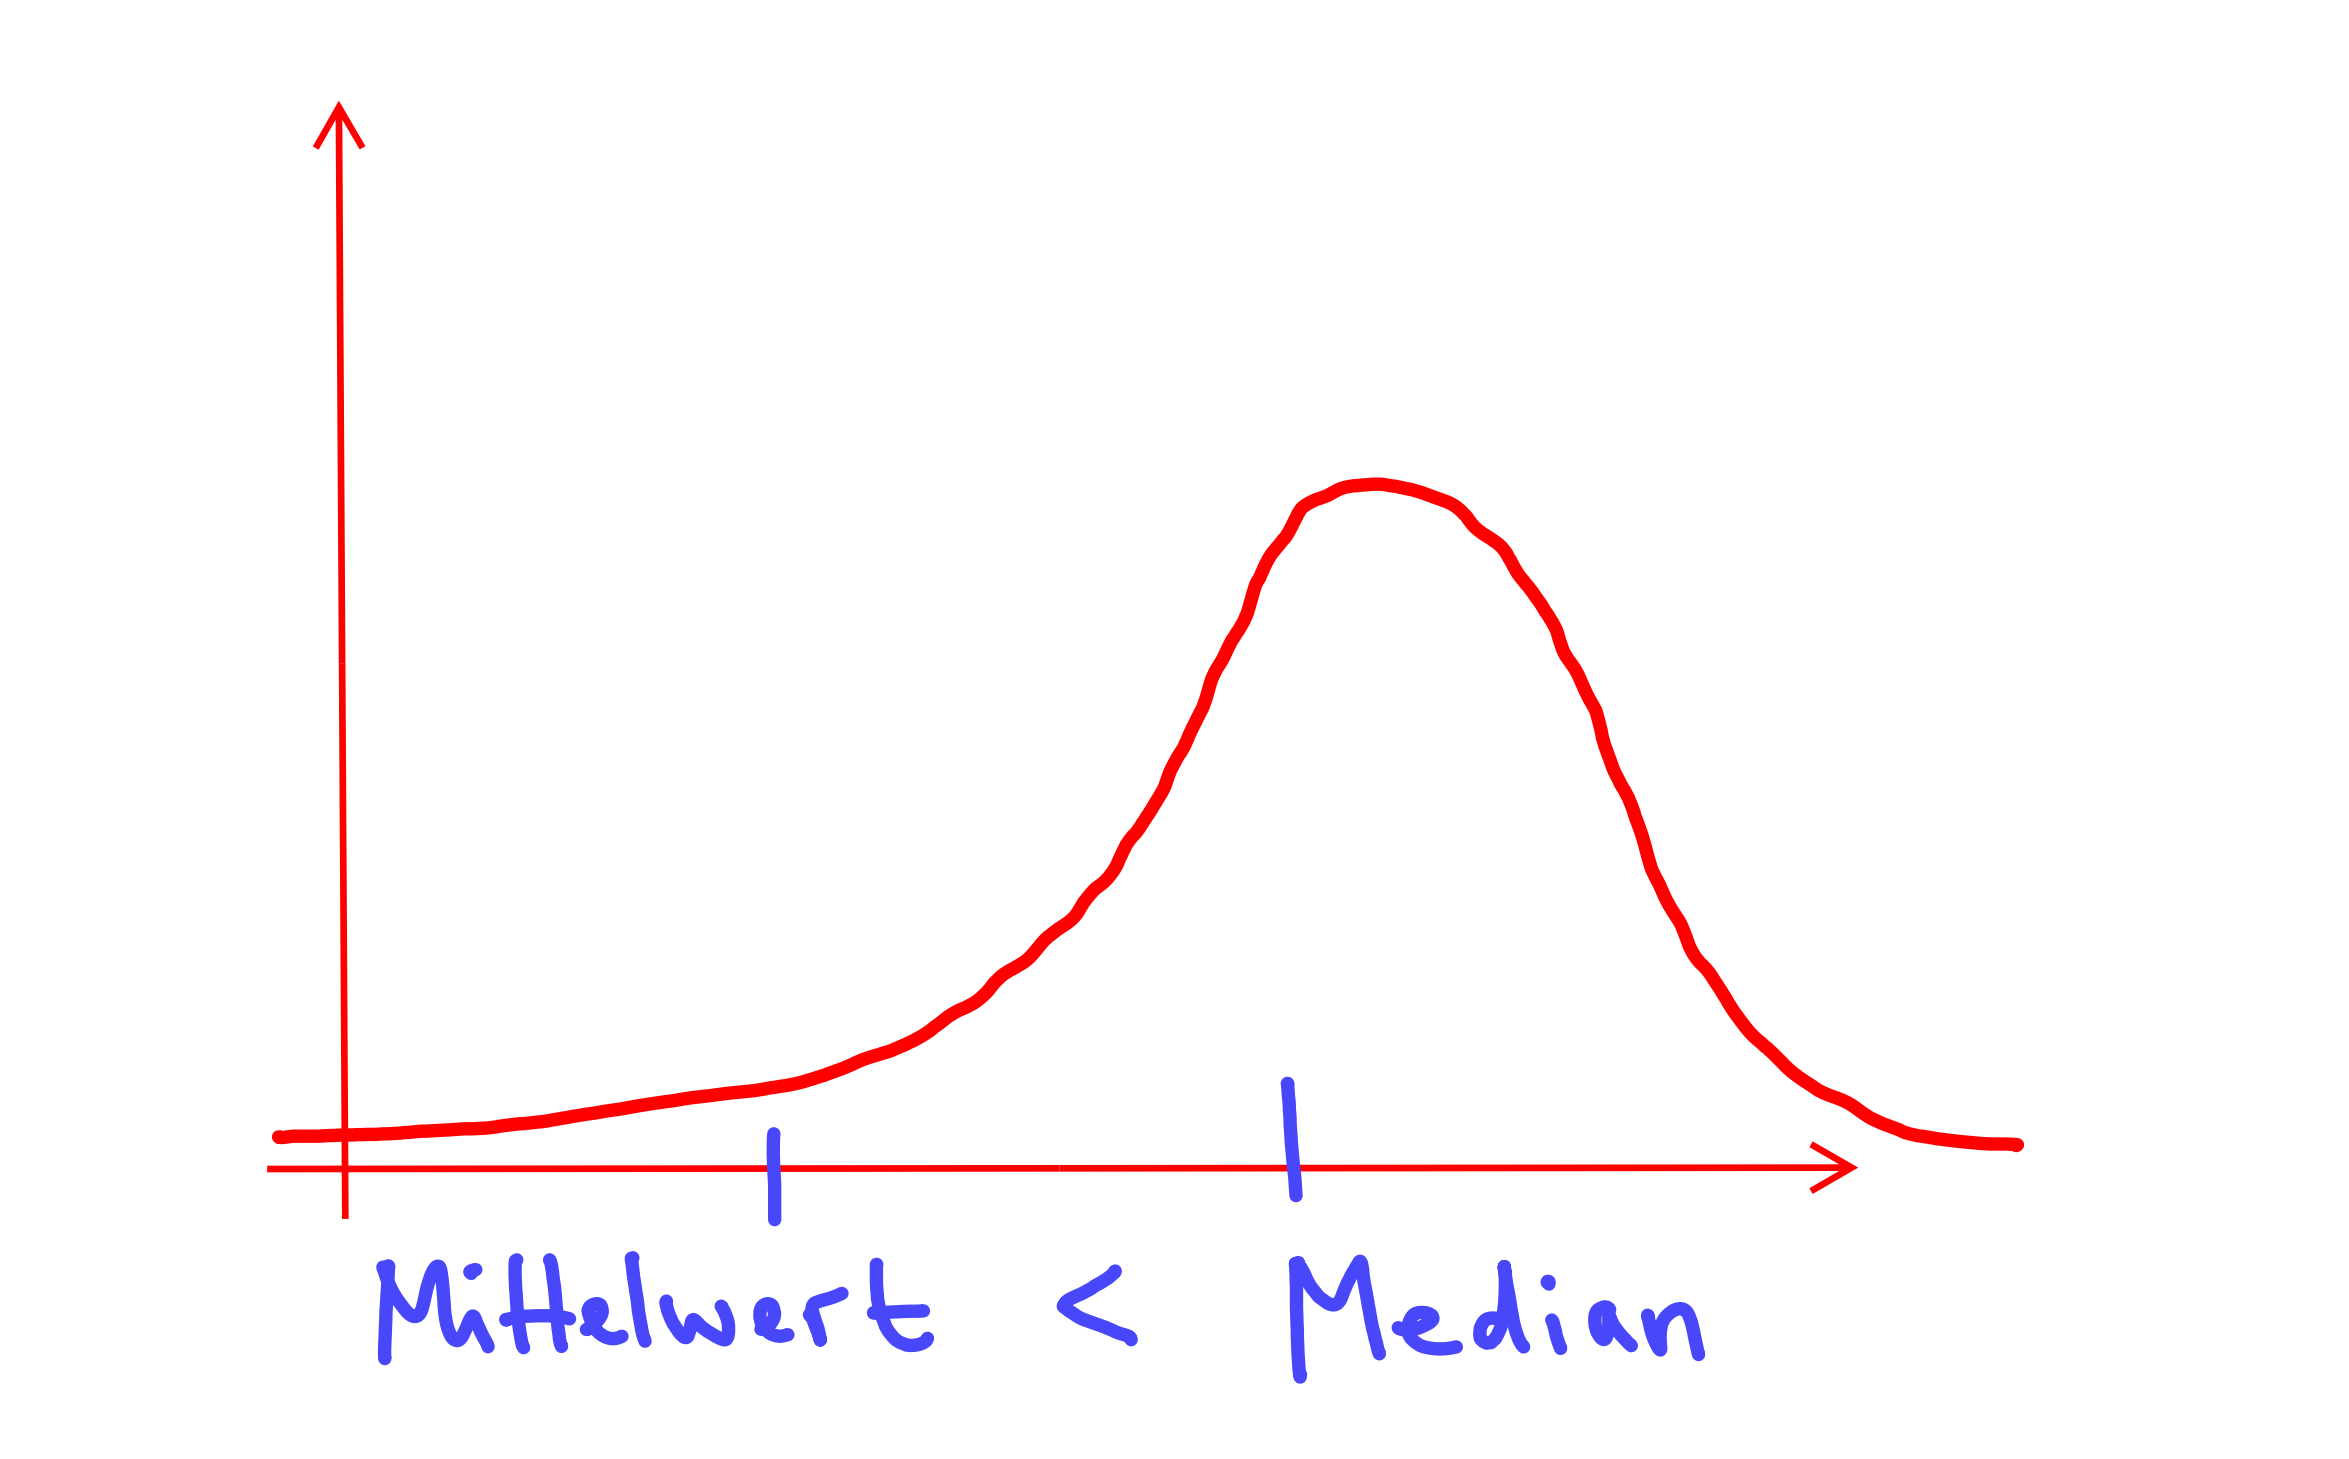
\includegraphics[scale=0.15]{3.png}  \\ 
		$g_m>0$ & $g_m\approx0$ & $g_m<0$
	\end{tabular} 
\end{center}
Momentenkoeffizient der Schiefe
$$g_m = \frac{1}{n} \sum_{i=1}^{n} \left(  \frac{x_i - \bar{x}}{s} \right)^3 $$
\end{frame}
	
\begin{frame}
    Beispiel: linkssteile / rechtsschiefe Verteilung
    \vspace{-0.7cm}
	\begin{center}
		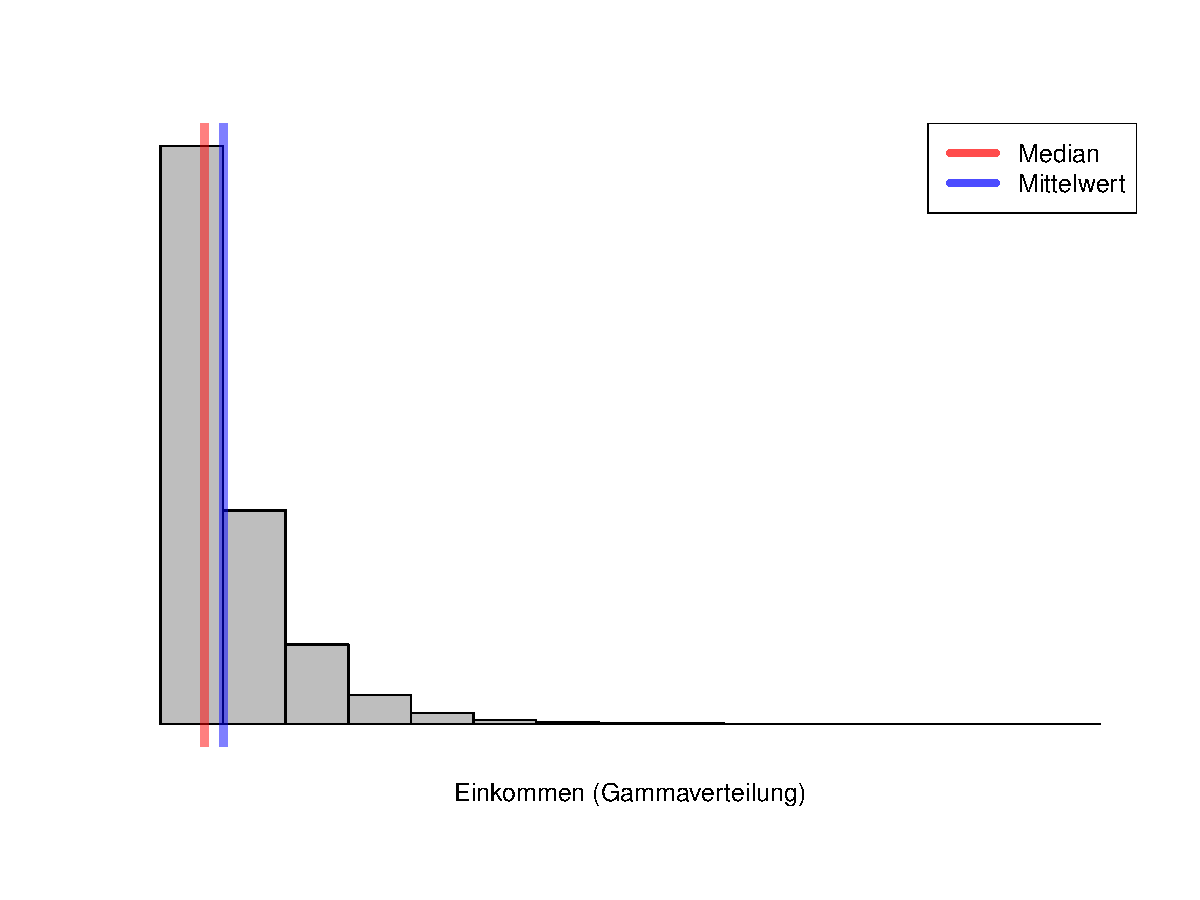
\includegraphics[scale=0.5]{1.pdf}
	\end{center}
\end{frame}

\begin{frame}
	Beispiel: symmetrische Verteilung
	\vspace{-0.7cm}
	\begin{center}
		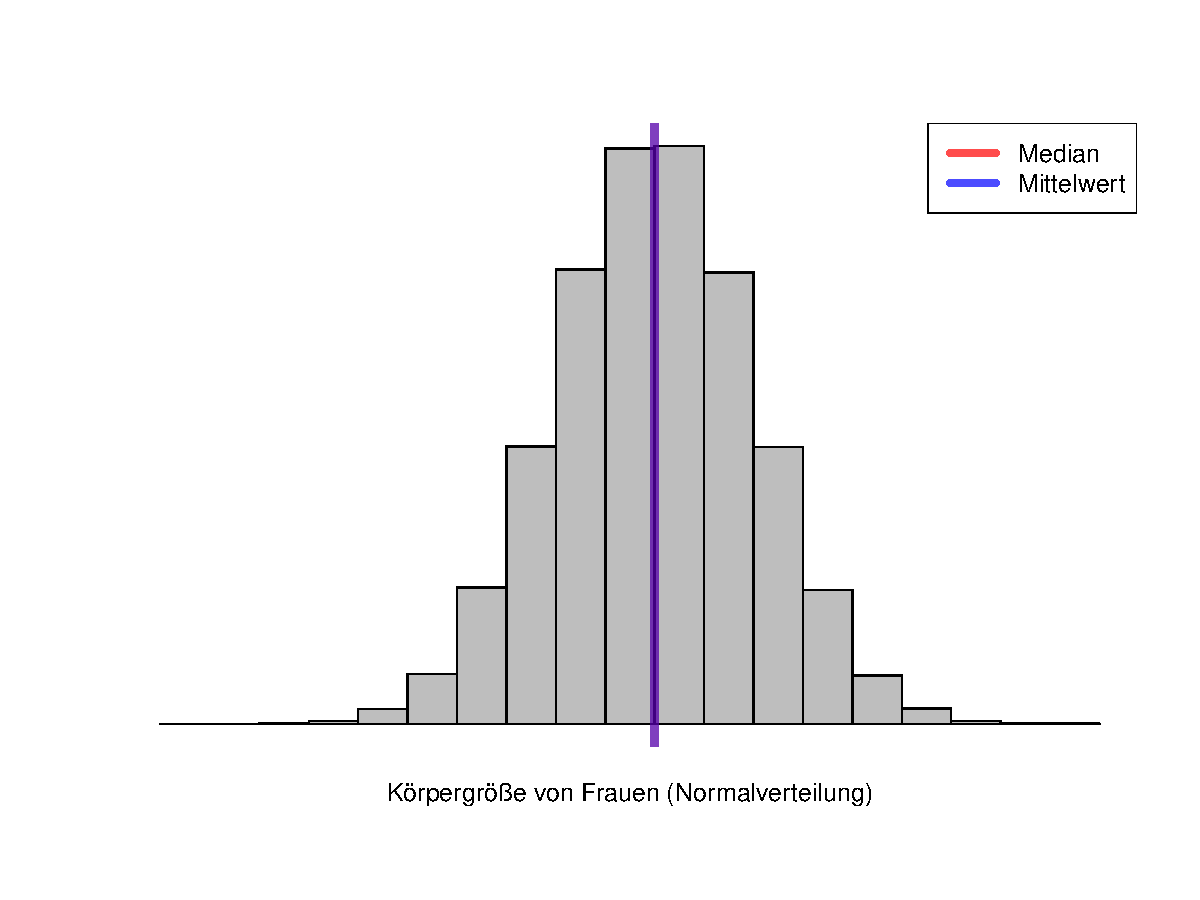
\includegraphics[scale=0.5]{2.pdf}
	\end{center}
\end{frame}

\begin{frame}
	Beispiel: rechtssteile / linksschiefe Verteilung
	\vspace{-0.7cm}
	\begin{center}
		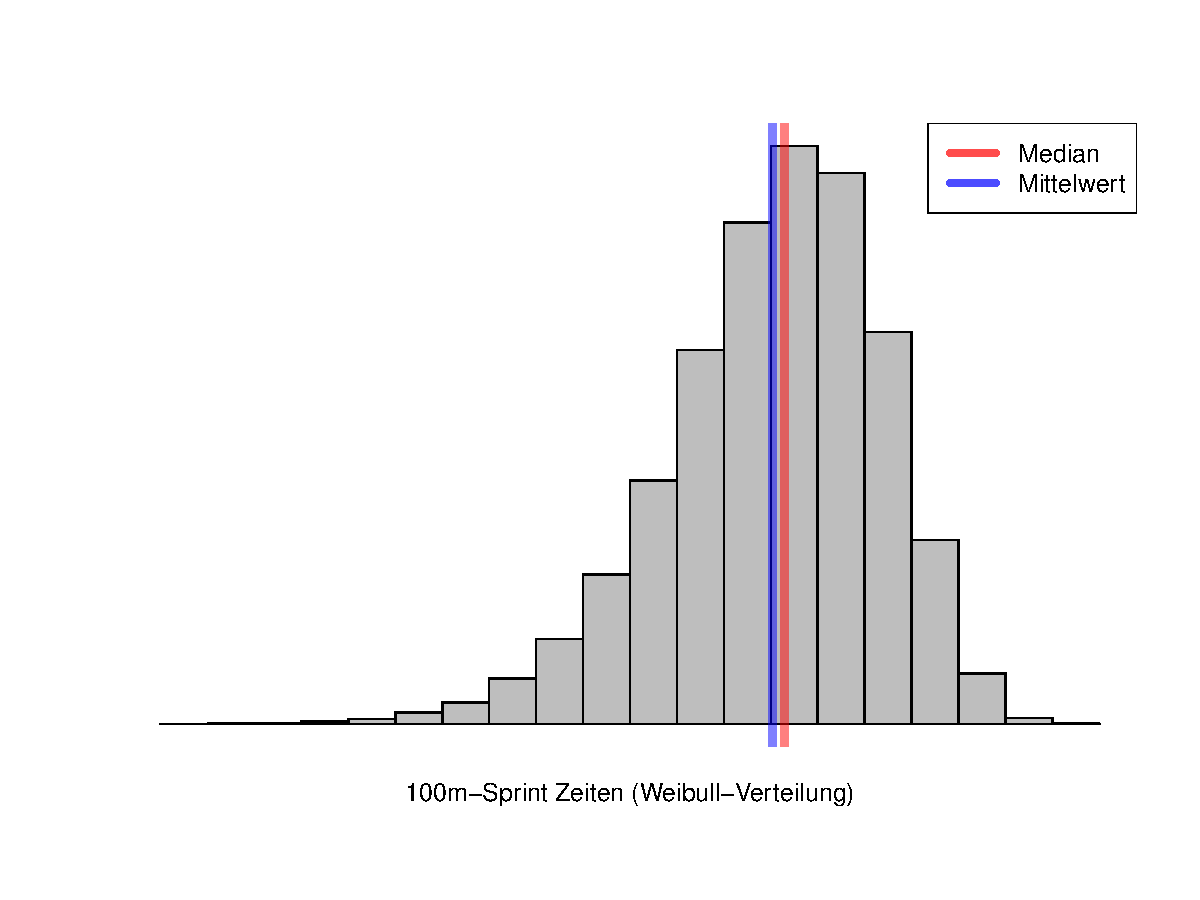
\includegraphics[scale=0.5]{3.pdf}
	\end{center}
\end{frame}

\end{document}